\documentclass[11pt,dvipsnames]{article} % {{{

\usepackage{geometry}
\geometry{total={170mm,240mm}, left=20mm, top=20mm}

\usepackage[utf8]{inputenc}

\usepackage{physics} 
\usepackage{siunitx} 
\usepackage{enumerate} 
\usepackage{pgfplots}
\usepackage{physics}
% To add figures
\usepackage{graphicx}
% Path to figures
\graphicspath{ {../images/} }

\usepackage{pgfplotstable}
\usepackage{tikz,pgfplots}
\usepackage{amsmath} 
\usepackage{xcolor}
\usepackage{float}
\usepackage{amsfonts}
\newcommand{\pce}{PCE}
\usepackage{dsfont}
\usepackage{amssymb}
%\usepackage{bbold}


\newcommand{\fref}[1]{fig.~\ref{#1}}  
\newcommand{\tref}[1]{table~\ref{#1}}
\newcommand{\Fref}[1]{Fig.~\ref{#1}}  
\newcommand{\Tref}[1]{Table~\ref{#1}}
\newcommand\dsone{\mathds{1}}

\newcommand{\R}{\mathcal{R}}
\newcommand{\psii}{\psi_i}
\newcommand{\Pk}[1]{\ket{\psi_{#1} }}
\newcommand{\Pb}[1]{\bra{\psi_{#1} }}
\newcommand{\pk}{\ket{\psi}}
\newcommand{\M}{\mathcal{M}^{(N)}}
\newcommand{\E}{\mathcal{E}}
\newcommand{\Ej}[1]{\E_{j_{#1}}}
\newcommand{\id}[1]{\qty(\1-\E_{j_{#1}})}
\newcommand{\Erho}{\mathcal{E}(\rho)}
\newcommand{\1}{\mathds{1}}
\newcommand{\ten}{\otimes}
\newcommand{\h}[1]{\colorbox{Yellow}{#1}}
\newcommand{\hi}{\mathcal{H}}
\newcommand{\txt}[1]{\text{#1}}
\newcommand{\here}{\h{\hspace{15cm}} }
\newcommand{\rhoi}{\dyad{\psii}{\psii}}
\newcommand{\ind}[2]{ {{}^{#1}_{#2}} }
\newcommand{\rc}[1]{r_{#1}}
\newcommand{\pauli}[2]{\sigma_{#1}\otimes\sigma_{#2}}
\newcommand{\Er}{\E_{\mathcal{R}} }
\newcommand{\PCE}[1]{\mathsf{PCE}_\mathsf{#1}}
\newcommand{\ot}{\otimes}
\usepackage[]{lineno}  \linenumbers
\setlength\linenumbersep{3pt}
	

\usepackage{fancybox}
\usepackage{colortbl}
\usepackage{amsbsy}
\usepackage[draft,inline,nomargin]{fixme} \fxsetup{theme=color}
\FXRegisterAuthor{cp}{acp}{\color{blue}CP}
\FXRegisterAuthor{ja}{aja}{\color{RedViolet}JA}
\FXRegisterAuthor{dd}{ddg}{\color{red}DD}
% }}}
\begin{document}
% Titulo y otros {{{
\title{Pauli component erasing operations} 
%Title should be concise and to the point  
\author{J. A. de León, C. Pineda, D. Dávalos, A. Fonseca}
\date{\today}  
\maketitle
\abstract{We study operations that act on the density matrix of $n$-qubits
systems and erase its projections onto tensor products of Pauli matrices. We
call this operations Pauli component erasing (PCE). We seek to characterize 
the subset of PCE operations that are quantum channels. We have solved 
analytically the complete positivity of a more general kind of operations.
Our numerical results suggest that PCE quantum channels have an algebraic structure.}

% }}}
% Intro 
\section*{Introduction} % {{{
The density matrix is an adequate tool to describe the kinematics 
of open quantum systems. An operator $\rho$ represents a quantum state and
is called a density operator if it is (1) of unitary trace, (2) Hermitian, and 
(3) positive. The density matrix of a system of $n$ qubits can be written as 
\begin{align}\label{eq:rho_nQubits_pauliBasis}
\rho =\frac{1}{2^n} \sum_{j_1,\ldots,j_n=0}^3r_{j_1,\ldots,j_n}
\sigma_{j_1}\otimes \ldots \otimes \sigma_{j_n},
\hspace{2cm} r_{0,\ldots,0}=1,
\end{align}
where $\sigma_{j_k}$ are the Pauli matrices (with $\sigma_0$ as $\1$)
and $r_{j_1,\ldots,j_n}$ the projections of $\rho$ onto each element of 
the basis of tensor products of Pauli matrices. We may refer to the 
$r_{j_1,\ldots,j_n}$ as the ``Pauli components'' of the density matrix 
of a system of qubits.  The component $r_{0,\ldots,0}$
must be equal to one in order for $\rho$ to satisfy $\Tr \rho =1$. 

Let us now define what a Pauli component erasing (PCE) operation is. 
A linear operation $\mathcal{E}$ is a PCE operations if it 
acts on a density matrix of $n$ qubits and transforms its Pauli components as
\begin{align}\label{eq:PCE-definition}
r_{j_1,\ldots,j_n} \longmapsto \tau_{j_1,\ldots,j_n}r_{j_1,\ldots,j_n}
\hspace{1cm} \tau_{j_1,\ldots,j_n}=0,1,
\hspace{1cm} \tau_{0,\ldots,0}=1.
\end{align}
In simple words, a PCE operation leaves invariant or erases the Pauli 
components of a density matrix of $n$ qubits.
%\begin{align}
%  \rho = \frac{1}{2^n}\1 + \sum _{i=1}^{2^{2n}-1}\tau _i\sigma _i,
%	\label{rho}
%\end{align}
%where the $\sigma _i$s are tensor products of Pauli 
%matrices, which together with the identity, form a orthogonal basis in the space of
%$2^n\times 2^n$ matrices. Thus the $\tau_i$s are the projections of $\rho$ onto
%each element of this basis, using the Hilbert-Schmidt inner product.

In this work, we are interested in studying the subset of PCE operations
that are quantum channels. 
Let us discuss briefly the definition of a quantum channel.
A quantum channel is a linear operation that acts on a density matrix $\rho$
that is completely positive and preserves the trace of $\rho$. The complete
positivity is a condition that captures the non-locality of 
quantum mechanics. One standard definition is the following: an operation
$\mathcal{E}$ is completely positive if and only if $\mathcal{E}\otimes\1_k$
is a positive operator for every possible dimension $k$. In other words, 
$\mathcal{E}\otimes\1_k$ must be an operator that maps positive 
matrices onto positive matrices, including the entangled states between 
the system which $\mathcal{E}$ acts on and an arbitrary system 
which $\1_k$ acts on. In fact, the complete positivity of an operation 
$\mathcal{E}$ may be evaluated by checking that the maximally 
entangled pure state between the system and an identical copy is mapped 
by $\mathcal{E}\otimes\1$ onto a positive matrix, \textit{i.e.}
$\qty(\mathcal{E}\otimes\1)\qty[\dyad{\phi^+}{\phi^+}]\geq 0$, with 
$\dyad{\phi^+}{\phi^+}$ the maximally entangled pure state state.

We're interested in characterizing the quantum PCE channels.
For 1 qubit the picture of our problem is easy to understand given that 
the Pauli components are the components of a vector in the Bloch sphere,
the so-called Bloch vector. 
As an example, let us consider a map that erases any single
component of the Bloch vector. Geometrically, this map collapses 
the Bloch ball into a disk. This operation is not completely positive, and
therefore is not a quantum channel.  However, erasing two components yields 
a quantum channel.

So far, we have analytically solved the diagonalization for 
complete positivity of a more general class of operations than the PCE 
and have numerically found the all the PCE quantum channels up to 
4-qubit systems. We have made several observations from our results, but
we have not been able to prove them analytically and connect them 
all as a consequence of the mathematical characterization we desire
to find of the PCE quantum channels.
%
%So far, we have evaluated complete positivity numerically, we have obtained all 1 and
%2 \pce{} operations. Whereas for $3$ qubits systems we have numerically analyzed
%only maps that leave invariant 1, 2, 3, 4, and 64 Pauli components in $\rho$.
%Nonetheless, we have strong indications that only maps that leave invariant 8
%components are needed to analyze in order to find the complete set of 3-qubit
%PCE channels.
% }}}
\section*{Results} % {{{

\subsection*{Diagonalization of the Choi matrix}
Due to the fact that the Pauli matrices and the identity form a basis of the Hilber-Shmidt space, the state of a qubit may be written as
% 
\begin{equation}
 \hat{\rho}=\frac{1}{2}\sum_{j,k=0}^1r_{jk}\hat{v}_{jk},
\end{equation}
%
where $\hat{v}_{00}=\dsone$, $\hat{v}_{01}=\hat{\sigma}_x$, $\hat{v}_{10}=i\hat{\sigma}_y$ and $\hat{v}_{11}=\hat{\sigma}_z$.
% 
Rewriting $\hat{\rho}$ in ``vector" notation, we have
%
\begin{equation}
 \vec{\rho}=\frac{1}{2}\sum_{jk=0}^1r_{jk}\vec{v}_{jk},
\end{equation}
%
The action of a quantum operation $\hat{M}$ (in its matrix form), capable of modifying each one of the coefficients $r_{jk}$ independently may be written as
%
\begin{equation}
 \hat{M}\vec{\rho}=\frac{1}{2}\sum_{jk=0}^1\tau_{jk}r_{jk}\vec{v}_{jk}.
\end{equation}
%
In our particular case (PCE operations), $\tau_{jk}=\{0,1\}$. 

In order to determine whether any specific operation, characterized by the set of coefficients $\{\tau_{jk}\}$ corresponds to a quantum channel, we must ensure that the eigenvalues associated to the Choi matrix are non-negative. For this, let write $\hat{M}$ in the vector Pauli basis
%
\begin{equation}
 \hat{M}=\sum_{jk=0}^1\tau_{jk}~\vec{v}_{jk}\vec{v}_{jk}^\intercal.
 \label{EQA1}
\end{equation}
%
On the other hand, it is easy to show that the elements of the computational and Pauli bases are related by $\vec{u}=\hat{T}\vec{v}$
\begin{equation}
\vec{u}=\begin{pmatrix}
\hat{u}_{00} \\ \hat{u}_{01} \\ \hat{u}_{10} \\ \hat{u}_{11}
\end{pmatrix}=\frac{1}{2}\begin{pmatrix}
1 & 0 & 0 & 1\\
0 & 1 & 1 & 0\\
0 & 1 & -1 & 0\\
1 & 0 & 0 & -1
\end{pmatrix} \begin{pmatrix}
\hat{v}_{00} \\ \hat{v}_{01} \\ \hat{v}_{10} \\ \hat{v}_{11}
\end{pmatrix},
\end{equation}
% 
where $\hat{u}_{jk}=\dyad{j}{k}$. The inverse relation reads $\vec{v}=\hat{S}\vec{u}$
\begin{equation}
\vec{v}=\begin{pmatrix}
\hat{v}_{00} \\ \hat{v}_{01} \\ \hat{v}_{10} \\ \hat{v}_{11}
\end{pmatrix}=\begin{pmatrix}
1 & 0 & 0 & 1\\
0 & 1 & 1 & 0\\
0 & 1 & -1 & 0\\
1 & 0 & 0 & -1
\end{pmatrix} \begin{pmatrix}
\hat{u}_{00} \\ \hat{u}_{01} \\ \hat{u}_{10} \\ \hat{u}_{11}
\end{pmatrix}.
\end{equation}
% 
Thus, for this ``indexing choice" of the elements of the bases, the transformation matrices satisfy $\hat{S}=2\hat{T}$. Then one can relate the bases elements in a compact form as
% 
\begin{equation}
 \vec{v}_{jk}=\sum_{mn=0}^1S_{mn}^{(jk)}\vec{u}_{mn},
\end{equation}
% 
by substituting this in Eq. \ref{EQA1} we get $\hat{M}$ in the computational basis
% 
\begin{align}
 \hat{M}=&\sum_{jk=0}^1\tau_{jk}~\left(\sum_{mn=0}^1S_{mn}^{(jk)}\vec{u}_{mn} \right) \left(\sum_{pq=0}^1S_{jk}^{(pq)}\vec{u}^\intercal_{pq} \right),\\
 =&\sum_{mnpq=0}^1\left(\sum_{jk=0}^1 S_{mn}^{(jk)}S_{jk}^{(pq)}  \tau_{jk} \right) \vec{u}_{mn}\vec{u}^\intercal_{pq}.\\
 &\sum_{mnpq=0}^1 M_{\substack{mn\\pq}} ~\vec{u}_{mn}\vec{u}^\intercal_{pq}.
\end{align}
% 
In order to obtain the Choi matrix $\hat{M}^c$, we must perform the reshuffling operation on $\hat{M}$, i.e. $M_{\substack{mn\\pq}} \to M_{\substack{mp\\nq}}$ \cite{bengtsson_zyczkowski_2017}. In this way, $\hat{M}^c$ holds

\begin{equation}
\hat{M}^c=\sum_{mnpq=0}^1\left(\sum_{jk=0}^1 S_{mp}^{(jk)}S_{jk}^{(nq)}  \tau_{jk} \right) \vec{u}_{mn}\vec{u}^\intercal_{pq}.
\end{equation}
%
Back to the Pauli basis, we have
%
\begin{equation}
 \hat{M}^c=\sum_{\mu\nu\alpha\beta=0}^1\left\{\sum_{jk=0}^1\left[\sum_{mnpq=0}^1S_{mp}^{(jk)}S_{jk}^{(nq)}T_{\mu\nu}^{(mn)}T_{pq}^{(\alpha\beta)}\right]\tau_{jk}\right\}\vec{v}_{\mu\nu}\vec{v}_{\alpha\beta}^\intercal.
\end{equation}
%
By taking into account the relation between the transformation matrices $T_{\mu\nu}^{(mn)}=\frac{1}{2}S_{\mu\nu}^{(mn)}$, $\hat{M}^c$ reads
%
\begin{equation}
 \hat{M}^c=\frac{1}{4}\sum_{\mu\nu\alpha\beta=0}^1\left\{\sum_{jk=0}^1\left[\sum_{mnpq=0}^1S_{mp}^{(jk)}S_{jk}^{(nq)}S_{\mu\nu}^{(mn)}S_{pq}^{(\alpha\beta)}\right]\tau_{jk}\right\}\vec{v}_{\mu\nu}\vec{v}_{\alpha\beta}^\intercal.
\end{equation}
%
By noticing that $S_{mn}^{(jk)}=(-1)^m\delta_{jm}\delta_{kn}+\delta_{j,m\oplus 1}\delta_{k,n\oplus 1}$, and after several steps it is possible to show that 
% 
\begin{equation}
\frac{1}{4}\sum_{jk=0}^1\left[\sum_{mnpq=0}^1S_{mp}^{(jk)}S_{jk}^{(nq)}S_{\mu\nu}^{(mn)}S_{pq}^{(\alpha\beta)}\right]\tau_{jk}=\frac{1}{2}\delta_{\nu\beta}\delta_{\mu\alpha}\sum_{jk=0}^1(-1)^{j\mu\oplus k\nu}\tau_{jk},
\label{EQAL2}
\end{equation}
% 
after substituting, the Choi matrix reduces to
%
\begin{align}
 \hat{M}^c=&\frac{1}{2}\sum_{\mu\nu\alpha\beta=0}^1\left\{\delta_{\nu\beta}\delta_{\mu\alpha}\sum_{jk=0}^1(-1)^{j\mu\oplus k\nu}\tau_{jk}\right\}\vec{v}_{\mu\nu}\vec{v}_{\alpha\beta}^\intercal,\\
 =&\frac{1}{2}\sum_{\mu\nu=0}^1\left\{\sum_{jk=0}^1(-1)^{j\mu\oplus k\nu}\tau_{jk}\right\}\vec{v}_{\mu\nu}\vec{v}_{\mu\nu}^\intercal.
\end{align}
%
As it can be seen, this is the diagonal form of the Choi matrix. Thus, its 4 eigenvalues may be written in a compact form as
%
\begin{equation}
\lambda_{\mu\nu}=\frac{1}{2}\sum_{jk=0}^1(-1)^{j\mu\oplus k\nu}\tau_{jk},
\end{equation}
%
where $\mu,\nu=\{0,1\}$. Note in addition that this is in agreement with results already known in literature.

By following the same steps we can obtain the generalization to the $N$-qubits case. First of all note that $\hat{M}$ may be written as
%
\begin{equation}
 \hat{M}=\sum_{\vec{k}\vec{l}}\tau_{\vec{k}\vec{l}}~\vec{v}_{\vec{k}\vec{l}}\vec{v}_{\vec{k}\vec{l}}^\intercal,
%  \label{EQA1}
\end{equation}
% 
where
% 
\begin{equation}
 \vec{v}_{\vec{k}\vec{l}}=\vec{v}_{k_1l_1}\otimes\dots\vec{v}_{k_Nl_N}=\bigotimes_{j=1}^N\vec{v}_{k_jl_j}.
%  \label{EQA1}
\end{equation}
% 
Let write $\hat{M}$ in the $N$-qubits computational basis
% 
\begin{align}
 \hat{M}=&\sum_{\vec{k}\vec{l}\vec{p}\vec{q}}\left\{\sum_{\vec{m}\vec{n}} \left[ \prod_{i=1}^N S_{k_il_i}^{(m_in_i)}S_{m_in_i}^{(p_iq_i)} \right] \tau_{\vec{m}\vec{n}} \right\} \bigotimes_{j=1}^N\vec{u}_{k_jl_j}\vec{u}_{p_jq_j}^\intercal,\\
 =&\sum_{\vec{k}\vec{l}\vec{p}\vec{q}} M_{\vec{k}\vec{l}\vec{p}\vec{q}} ~\bigotimes_{j=1}^N\vec{u}_{k_jl_j}\vec{u}_{p_jq_j}^\intercal.
\end{align}
% 
After reshuffling ($M_{\vec{k}\vec{l}\vec{p}\vec{q}}\to M_{\vec{k}\vec{p}\vec{l}\vec{q}}$) we can get the associated Choi matrix. Back to the Pauli basis, $\hat{M}^c$ holds
%
\begin{equation}
 \hat{M}^c=\frac{1}{4^N}\sum_{\vec{\mu}\vec{\nu}\vec{\alpha}\vec{\beta}}\left\{\sum_{\vec{m}\vec{n}}\left[\prod_{i=1}^N\left(\sum_{k_il_ip_iq_i=0}^1 S_{k_ip_i}^{(m_in_i)} S_{m_in_i}^{(l_iq_i)}S_{\mu_i\nu_i}^{(k_il_i)}S_{p_iq_i}^{(\alpha_i\beta_i)}\right)\right]\tau_{\vec{m}\vec{n}}\right\} \bigotimes_{j=1}^N\vec{v}_{\mu_j\nu_j}\vec{v}_{\alpha_j\beta_j}^\intercal.
\end{equation}
% 
Using the result in Eq. \ref{EQAL2} and after some steps it can be shown that
%
\begin{equation}
 \hat{M}^c=\sum_{\vec{\mu}\vec{\nu}}\left\{\frac{1}{2^N}\sum_{\vec{\alpha}\vec{\beta}}(-1)^{\vec{\mu}\cdot\vec{\alpha}\oplus \vec{\nu}\cdot\vec{\beta}}\tau_{\vec{\alpha}\vec{\beta}}\right\}\vec{v}_{\vec{\mu}\vec{\nu}}\vec{v}_{\vec{\mu}\vec{\nu}}^\intercal,
\end{equation}
% 
which is also the diagonal form of $\hat{M}^c$. In this way, the $4^N$ eigenvalues may be written compactly as
% 
\begin{equation}
 \lambda_{\vec{\mu}\vec{\nu}}=\frac{1}{2^N}\sum_{\vec{\alpha}\vec{\beta}}(-1)^{\vec{\mu}\cdot\vec{\alpha}\oplus \vec{\nu}\cdot\vec{\beta}}\tau_{\vec{\alpha}\vec{\beta}}.
\end{equation}
% 
From this we can evaluate whether the set of coefficients $\tau_{\vec{\alpha}\vec{\beta}}$ satisfy the condition to the specific operation be considered a quantum channel, i.e. $\lambda_{\vec{\mu}\vec{\nu}}\geq 0$, for all $\vec{\mu},\vec{\nu}$. Note moreover that the expression above may also be written as a tensor product of $4\times 4$ matrices $a$, as illustrated in the next subsection.

\subsection*{Complete positivity: analytical solution}
Let us discuss the role of the complete positivity condition of the 
PCE operations in our problem. We desire to find what are the 
characteristics that make a PCE operation a quantum channel.
In the way we defined a PCE operation in \eqref{eq:PCE-definition} it 
is a trace preserving operation. Therefore, the complete positivity is 
the only condition to be evaluated given a PCE operation. 

We found an analytical solution to evaluate the complete positivity.
Recall that an operation $\mathcal{E}$ is completely positive if 
$\qty(\mathcal{E}\otimes\1)\qty[\dyad{\phi^+}{\phi^+}]\geq 0$,
where $\dyad{\phi^+}{\phi^+}$ is the maximally entangled pure 
state between the system and another one that is an identical copy.
We showed that the diagonalization of 
$\qty(\mathcal{E}\otimes\1)\qty[\dyad{\phi^+}{\phi^+}]\geq 0$,
with $\mathcal{E}$ an operation that acts on the Pauli components of
a density matrix of $n$ qubits as
\begin{align} \label{eq:PauliOperation}
r_{j_1,\ldots,j_n}\longmapsto \tau_{j_1,\ldots,j_n}r_{j_1,\ldots,j_n},
\hspace{1.5cm} \tau_{0,\ldots,0}=1,
\end{align}
yields the eigenvalues $\lambda_i$
\begin{align} \label{eq:eigv_Choi_Pauli_operation}
\vec{\lambda}=\frac{1}{2^n}\qty(\bigotimes^na)\vec{\tau},
\end{align}
where 
\begin{align}
a=\mqty(1&1&1&1\\1&1&-1&-1\\1&-1&1&-1\\1&-1&-1&1)
\end{align} 
and the components of $\vec{\tau}$ the same ones in 
\eqref{eq:PauliOperation}. It is very important to realize that 
\eqref{eq:eigv_Choi_Pauli_operation} yields the diagonalization
not exclusively of a PCE operation. The difference between 
the definition of a PCE operation in \eqref{eq:PCE-definition}
and \eqref{eq:PauliOperation} is the relaxation in the value of 
the $\tau_{j_1,\ldots,j_n}$ (exclusively 0 or 1 for a PCE operation). 

\subsection*{PCE quantum channels}
In \fref{fig:pictorial-rep-rho} we introduce a pictorial representation 
for the identity map acting on a density matrix for systems 
of 1, 2 and 3 qubits,
respectively. It will be helpful to visualize the maps we are studying 
making use of this tool. We'll consider any little square or cube in blank
as a component erased in $\rho$ by the map. 
Red squares correspond to components of Bloch vectors of one-particle reduced density matrices,
blue squares to correlations between any pair of qubits, and
green squares to correlations between all qubits in the system for
the 3-qubits case.
In the following subsections we present the PCE channels for
1 and 2 qubits, and preliminary results for 3 qubits.
\begin{figure}[H] % {{{
	\centering
	\hfill \hfill
	
\includegraphics[height=2.5cm]	{tablero-1q}
	\hfill
	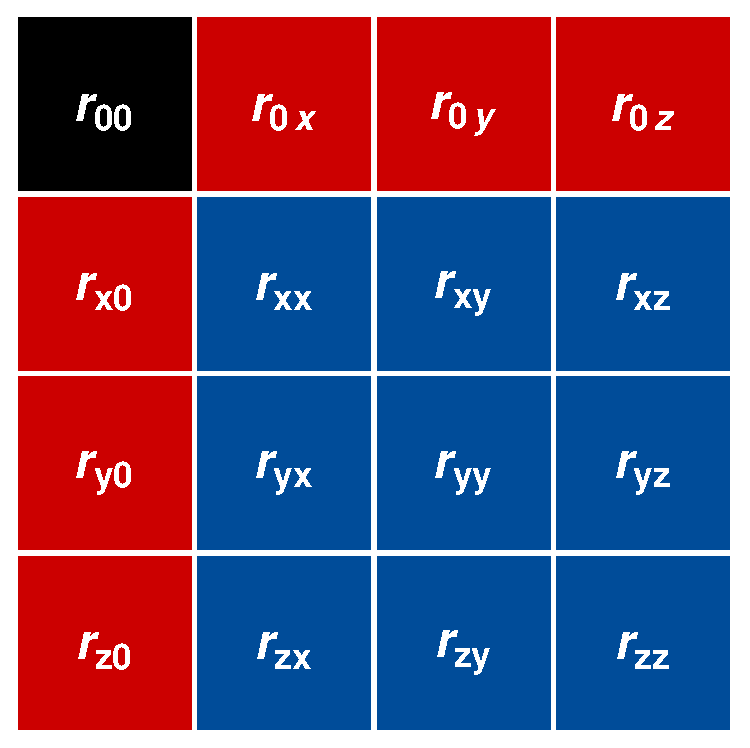
\includegraphics[width=2.5cm]{rho2q(2)}
	\hfill 
	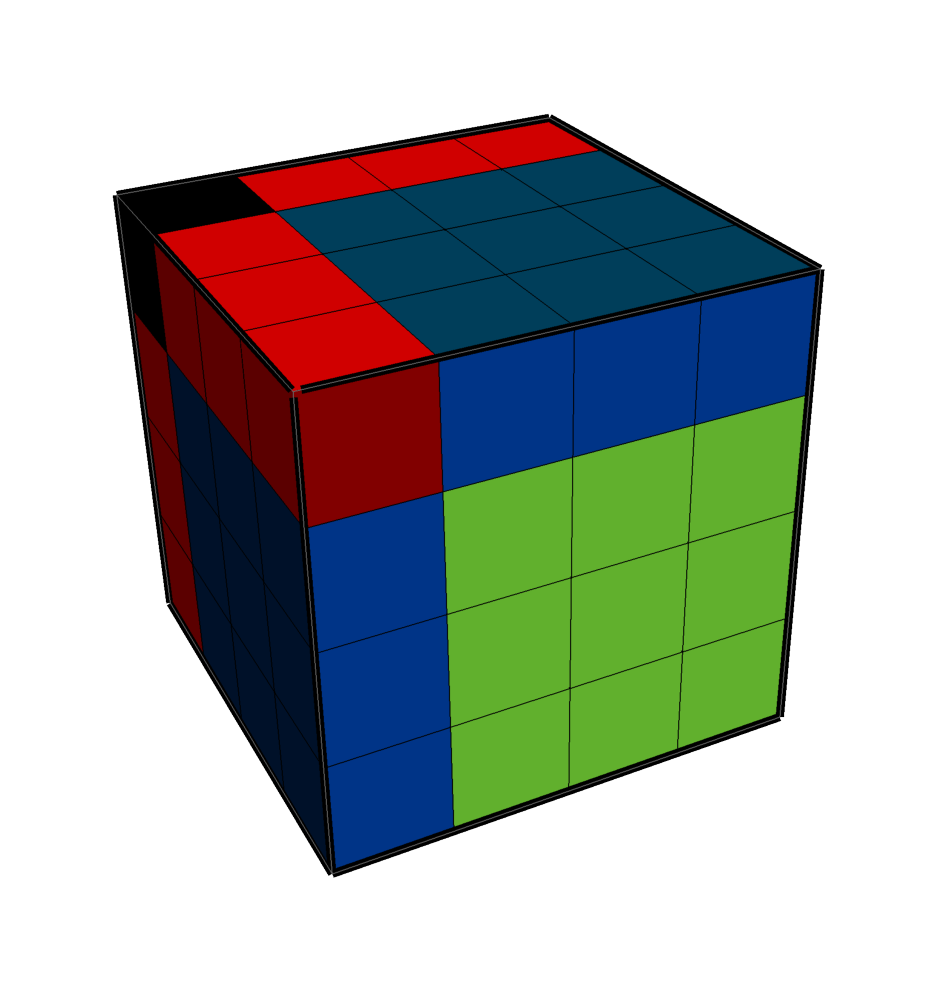
\includegraphics[width=2.5cm]{rho-3q}
	\hfill \hfill
	\caption{From left to right the identity map acting on
  an arbitrary density matrix of 1, 2 and 3 qubits, respectively. 
	Red squares correspond to components of local Bloch vectors,
	blue squares to correlations between any pair of qubits and
	green squares to correlations between all qubits in the system, for
	the 3-qubits case. }
	\label{fig:pictorial-rep-rho}
\end{figure} % }}}
\subsection*{1 qubit} % {{{
In \fref{fig:1q-ccs} we present the PCE channels for 1 qubit.
The first and last patterns represent identity 
and the total depolarizing channel. 
Patterns in between represent operations that map the Bloch 
sphere to a line on the Cartesian axes, respectively.
These three channels are equivalent via permutation
of the components $r_i$ of the Bloch vector.
\begin{figure}[H]% {{{
	\centering
	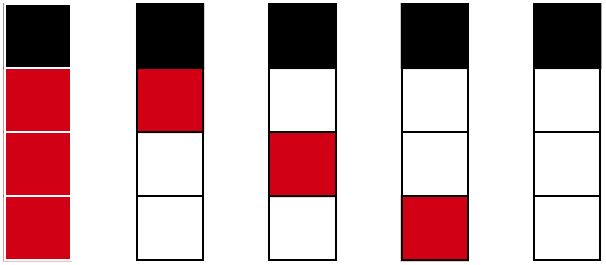
\includegraphics[width=5cm]{1q-CCs.png}
	\caption{
1-qubit PCE channels. From left to right patterns represent  
the following channels: identity,
mapping of the Bloch sphere to $x$ axis, $y$ axis, $z$ axis, 
and completely depolarizing (channel that maps every state 
to the maximally mixed).}
	\label{fig:1q-ccs}
\end{figure} % }}}
% }}}
\subsection*{2 qubits} % {{{
2-qubits PCE channels have been classified in equivalence classes 
(as shown from \fref{fig:2q-c1} to \fref{fig:2q-c16}), such
that elements in a class are connected by
\begin{enumerate}
	\item Particle swaps: Qubits in the system can be interchanged. Therefore
	if a map is a PCE channel for a certain arrangement 
	of qubits, then
	there are equivalent PCE channels acting on the system for all possible
	arrangements of qubits. In the pattern-picture this can be
	interpreted as transpositions.
	\item Exchange of axes labels: These operations correspond to permutations of rows and/or columns and are generally are not CPTP maps. For instance the swap of rows (or columns) result in reflections of the Bloch sphere of individual particles. Aside from that, it is clear that the physics of the erasure are the same.
%	The state of an individual
%	qubit may be rotated in such a way that components of its local Bloch
%	vector are swapped via permutations\cpnote{De acuerdo a lo que he pensado, esa frase no es cierta. 
%        Me gustaría discutir.}. PCE channels are equivalent
%	to these permutations.
%	In the pattern-picture this
%	is interpreted as permutations of rows or columns 1, 2 and 3.
\end{enumerate}

\begin{figure}[H] % {{{
	\centering
  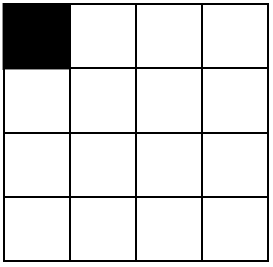
\includegraphics[height=1.2cm]{C16.png}
	\caption{C${}^{1}$}
	\label{fig:2q-c1}
\end{figure} % }}}

\begin{figure}[H] % {{{
	\begin{minipage}[c]{0.5\textwidth}
		\centering
	  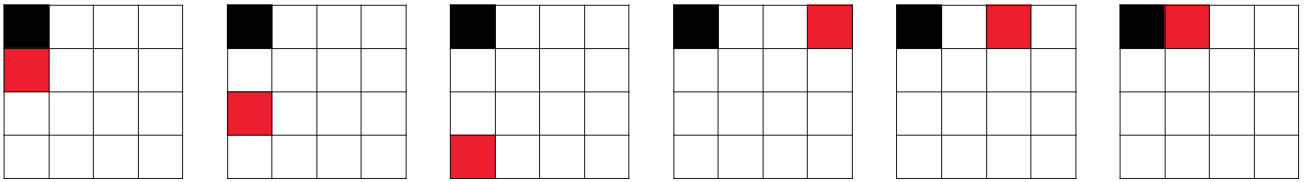
\includegraphics[width=.9\textwidth]{C12.png}
		\vspace{1.2cm}
		\caption{C${}_1^2$}
		\label{fig:equivalence_class_c12}
	\end{minipage}\hfill
	\begin{minipage}[c]{0.5\textwidth}
		\centering
	  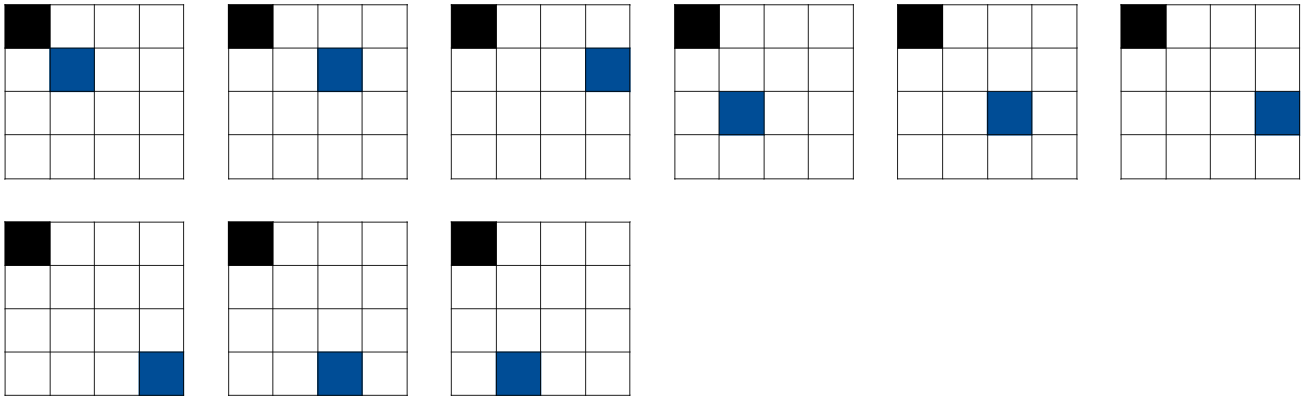
\includegraphics[width=.9\textwidth]{C22.png}
		\caption{C${}_2^2$}
		\label{fig:equivalence_class_22}
	\end{minipage}
\end{figure} % }}}

\begin{figure}[H] % {{{
	\begin{minipage}[c]{0.5\textwidth}
		\centering
	  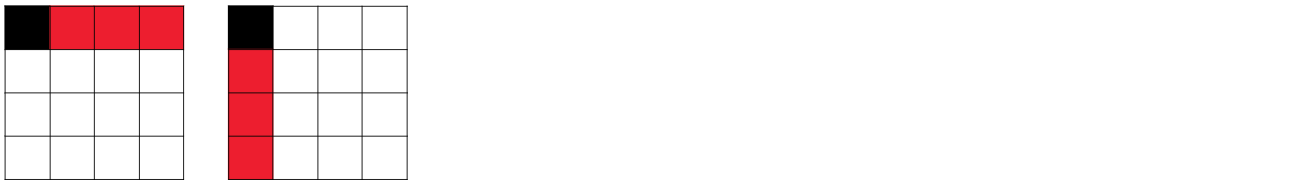
\includegraphics[width=.9\textwidth]{C14.png}
		\vspace{1.2cm}
		\caption{C${}_1^4$}
		\label{fig:equivalence_class_c14}
	\end{minipage}\hfill
	\begin{minipage}[c]{0.5\textwidth}
		\centering
	  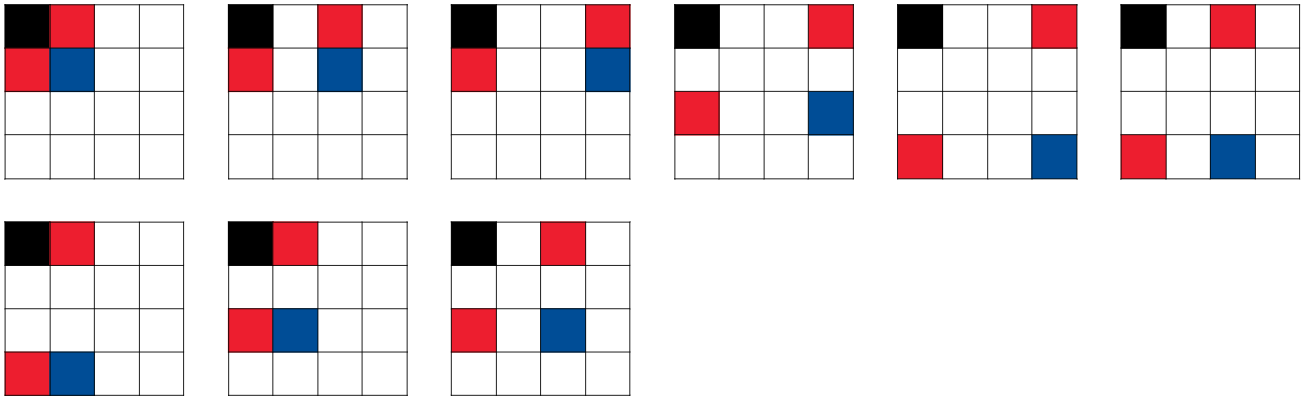
\includegraphics[width=.9\textwidth]{C24.png}
		\caption{C${}_2^4$}
		\label{fig:equivalence_class_c24}
	\end{minipage}\vfill
\begin{minipage}[c]{0.5\textwidth}
		\centering
	  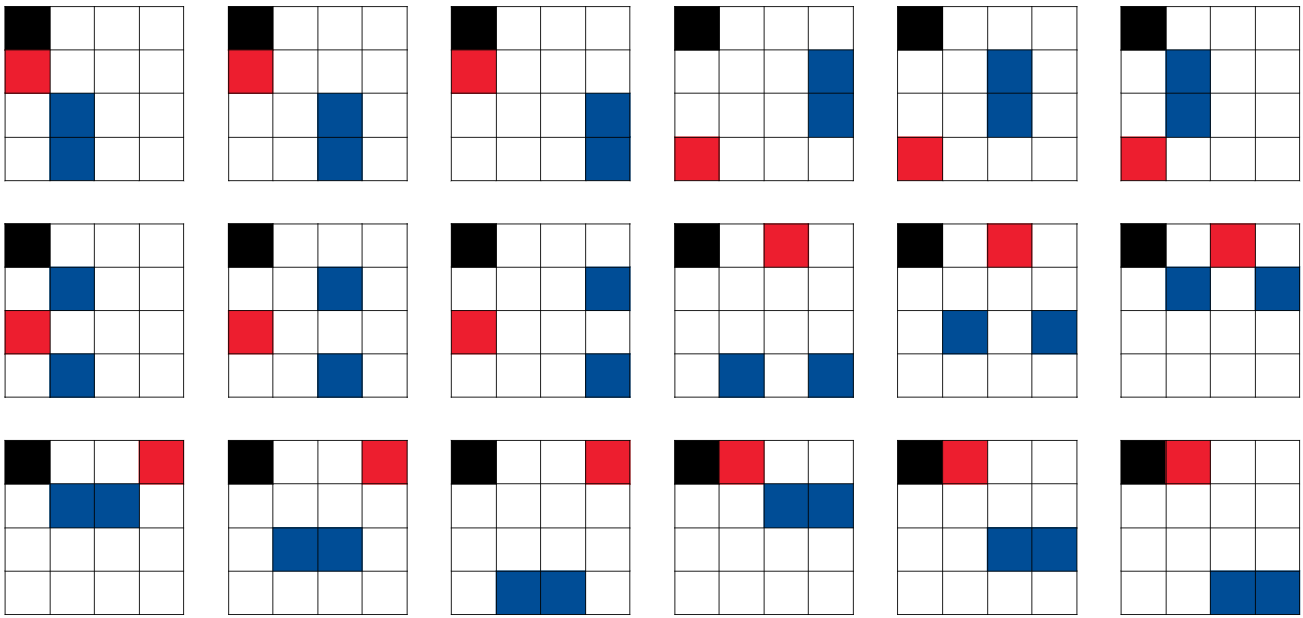
\includegraphics[width=.9\textwidth]{C34.png}
		\caption{C${}_3^4$}
		\label{fig:equivalence_class_c34}
	\end{minipage}\hfill
	\begin{minipage}[c]{0.5\textwidth}
		\centering
	  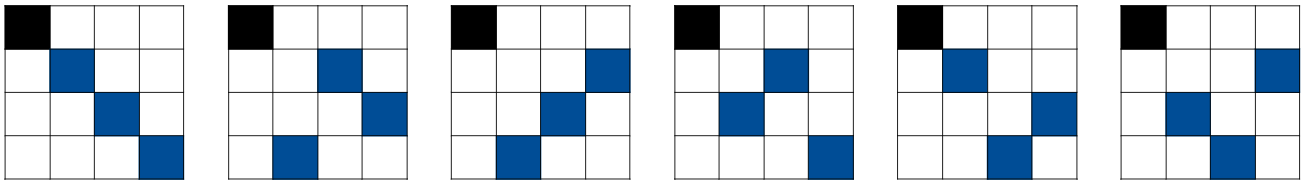
\includegraphics[width=.9\textwidth]{C44.png}
		\vspace{2.5cm}
		\caption{C${}_4^4$}
		\label{fig:equivalence_class_c44}
	\end{minipage}
\end{figure} % }}}

\begin{figure}[H] % {{{
	\begin{minipage}[c]{0.5\textwidth}
		\centering
	  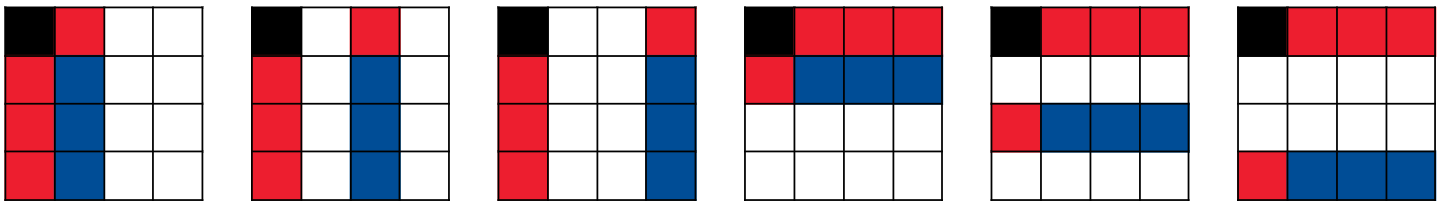
\includegraphics[width=.9\textwidth]{C18.png}
		\vspace{1.2cm}
		\caption{C${}_1^8$}
		\label{fig:equivalence_class_18}
	\end{minipage}\hfill
	\begin{minipage}[c]{0.5\textwidth}
		\centering
	  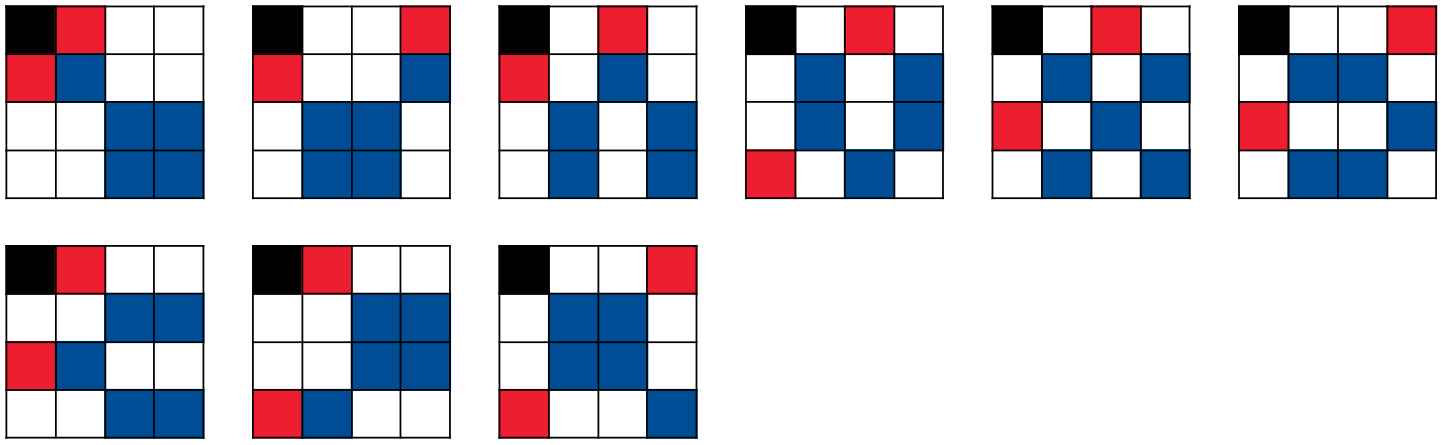
\includegraphics[width=.9\textwidth]{C28.png}
		\caption{C${}_2^8$}
		\label{fig:equivalence_class_28}
	\end{minipage}
\end{figure} % }}}

\begin{figure}[H] % {{{
	\centering
  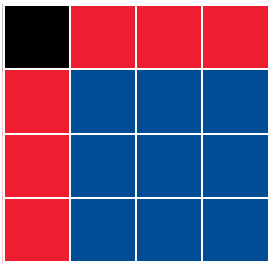
\includegraphics[height=1.2cm]{C0.png}
	\caption{C${}^{16}$}
	\label{fig:2q-c16}
\end{figure} % }}}

In general, our results exhibit the following features:
\begin{itemize}
\item (\textit{Power-of-2 rule})
Only a power-of-2 number of Pauli components in $\rho$ 
may be left invariant by a PCE channel. 
However, not only the number of Pauli components in $\rho$ 
to leave invariant determines complete positivity since
not all maps that leave $2^{k}$ Pauli components invariant in $\rho$
are quantum channels. For example, the pattern below corresponds 
to a map that is a potential element of C${}_2^4$ (\Fref{fig:2q-4c-2}).
Nevertheless, complete positivity is not satisfied 
and then the map is not a quantum channel. 
% \begin{figure}[H]
% 	\centering
% 	\includegraphics[height=2cm]{img/not-cc}
% \end{figure}
\begin{center}
	\includegraphics[height=2cm]{not-cc}
\end{center}

\item \textit{(Mirroring)}
The number of PCE quantum channels as a function of the number of Pauli 
components left invariant shows to be symmetric with respect to a
particular value. 
The number of PCE operations and quantum channels,
as a function of the number of Pauli components left invariant, 
for 2 qubits are shown in \tref{tab:qtm_channels}.

%The ratio PCE channels$:$PCE operations according to number of qubits 
%and number of Pauli components invariant are shown in 
%\fref{fig:CCs-by-components}.
%
%\begin{figure}[H]% {{{
%\centering	
%\footnotesize
%\begin{tabular}{c|ccccccccccc|c}
%% \bf{
%\textbf{qubits}  & \multicolumn{11}{c|}{PCE quantum channels${}:{}$PCE operations 
%($2^0,\ldots,2^{2n}$ Pauli components components invariant)} & total PCE \\
%\hline
%1 &&&&&$1:1$&$3:3$&$1:1$&&&&&5\\
%2 &&&&$1:1$&$15:15$&$35:455$&$15:6435$&$1:1$&&&&67\\
%3 &&&$1:1$&$63:63$&$651:39711$&?/$6\times 10^8$&
%$651:1\times 10^{14}$&$63:{9\times 10^{17}}$&$1:1$&&&?
%% }
%\end{tabular}
%\caption{First column shows the number of qubits in the system.  In the second
%column each position correspond to the number of components invariant ($2^0,
%2^1, \ldots, 2^{2n}$) and the numbers shown are the ratios of PCE channels
%and all possible maps according to the number of components invariant.  Finally, third column
%specifies the total number of PCE channels for a $n$-qubit system.}
%\label{fig:CCs-by-components}
%\end{figure} % }}}

\begin{table}[H]
\resizebox{\textwidth}{!}{%
\begin{tabular}{l|cccccccccccccccc}
\cline{2-17}
\multicolumn{1}{l|}{}                               & \multicolumn{16}{c|}{\textbf{Number of Pauli components left invariant}}                                                                                                                                                                                                                                                                                                                                                                                                                                                                                             \\[.5ex]
\multicolumn{1}{l|}{}                               & \multicolumn{1}{c}{\textbf{1}} & \multicolumn{1}{c}{\textbf{2}} & \multicolumn{1}{c}{\textbf{3}} & \multicolumn{1}{c}{\textbf{4}} & \multicolumn{1}{c}{\textbf{5}} & \multicolumn{1}{c}{\textbf{6}} & \multicolumn{1}{c}{\textbf{7}} & \multicolumn{1}{c}{\textbf{8}} & \multicolumn{1}{c}{\textbf{9}} & \multicolumn{1}{c}{\textbf{10}} & \multicolumn{1}{c}{\textbf{11}} & \multicolumn{1}{c}{\textbf{12}} & \multicolumn{1}{c}{\textbf{13}} & \multicolumn{1}{c}{\textbf{14}} & \multicolumn{1}{c}{\textbf{15}} & \multicolumn{1}{c|}{\textbf{16}} \\ \cline{2-17} 
\multicolumn{1}{c|}{\textbf{\# of PCE operations}}   & 1                               & 15                              & 105                             & 455                             & 1365                            & 3003                            & 5005                            & 6435                            & 6435                            & 5005                             & 3003                             & 1365                             & 455                              & 105                              & 15                               & 1                                \\[.4ex]
\multicolumn{1}{c|}{\textbf{\# of PCE qtm channels}} & 1                               & 15                              & 0                               & 35                              & 0                               & 0                               & 0                               & 15                              & 0                               & 0                                & 0                                & 0                                & 0                                & 0                                & 0                                & 1                               
\end{tabular}%
}
\caption{Tabla}
\label{tab:qtm_channels}
\end{table}
Let us focus only on the quantum channels:
\begin{table}[H]
\centering
\resizebox{.42\textwidth}{!}{%
\begin{tabular}{l|ccccc}
\cline{2-6}
\multicolumn{1}{l|}{}                               & \multicolumn{5}{c|}{\textbf{Number of $\boldsymbol{r_{ij}}$ inv.}} \\[.5ex]
\multicolumn{1}{l|}{}                               & \multicolumn{1}{c}{\textbf{1}} & \multicolumn{1}{c}{\textbf{2}} &  \multicolumn{1}{c}{\textbf{4}} & \multicolumn{1}{c}{\textbf{8}} &  \multicolumn{1}{c|}{\textbf{16}} \\ \cline{2-6} 
\multicolumn{1}{c|}{\textbf{\# of PCE qtm channels}} & 1                               & 15                               & 35                          & 15                        & 1                               
\end{tabular}%
}
\end{table}
We denote $f(k)$ the number of PCE quantum channels as a function
of the number $k$ of Pauli components left invariant. The number $k$
must be a power of 2.
In the case of 2 qubits, $f(k)$ is symmetric with respect to $k=4$. 
Our numerical results show that $f(k)$ is symmetric with respect
to $k=2^n$, in general. When 
considering only a power-of-2 Pauli components invariant,  
\tref{tab:qtm_channels} shows that this symmetry 
is not a property of the PCE operations, but only of the quantum channels.

\item \textit{($1:1$ correspondence)} There might be a 
$1:1$ correspondence between PCE quantum channels
that leave $2^k$ and $2^{2n-k}$ Pauli components invariant. 
That is to say in the 2-qubits case, 
PCE channels in Figs. \ref{fig:equivalence_class_c12}
and \ref{fig:equivalence_class_28} correspond to one 
PCE channel in Figs. \ref{fig:equivalence_class_18} and
\ref{fig:equivalence_class_28}. In fact, we've deduced from 
our numerical results the correspondence between PCE channels 
that leave 2 and the half the total Pauli components. For 2 qubits,
given the set $\{j_1,j_2 \}$ of indices of the Pauli component $r_{j_1,j_2}$ left
invariant, other than $r_{0,0}$, of every member in figs.
\ref{fig:equivalence_class_18} and \ref{fig:equivalence_class_18} one 
can one can find a single partner in figs. \ref{fig:equivalence_class_18} and
\ref{fig:equivalence_class_28} via
\begin{align}
\Phi_{j_1,j_2}=\E_{j_1}\ot\E_{j_2}+\qty(\1-\E_{j_1})\ot\qty(\1-\E_{j_2}),
\end{align}
where $\E_{j_l}$ are the first four 1-qubit PCE channels in 
\fref{fig:1q-ccs}, the identity and the 3 PCE operations that 
map the Bloch sphere to a line on every Cartesian axis. In general, 
a PCE quantum channel that leaves invariant $r_{0,\ldots,0}$ and 
$r_{j_1,\ldots,j_n}$ has a single PCE partner that leaves invariant 
half of the total Pauli components of the form 
\begin{align}
\Phi_{j_1,\ldots,j_n}=\sum_{i=0}^{i\leq n/2}\sum_{j\in \mathcal{S}_{2i}^n}
\bigotimes_{j_i=1}^n\Omega_{j_i},
\end{align}
with $\mathcal{S}_{2i}^n$ the set of all subsets with $2i$ elements 
from $\{1,2,\ldots,n\}$ and
\begin{align}
\Omega_{j_i}= \left\{ \begin{array}{rc}
             \E_{j_i}, & j_i \notin j \\
             \1 -\E_{j_i}, & j_i \in j.
             \end{array}
   \right.
\end{align}
We elaborate the 3-qubits and 4-qubits case. For 3 qubits, 
every PCE quantum channel that leaves invariant $r_{0,0,0}$ and 
$r_{j_1,j_2,j_3}$ has a PCE partner that leaves 32 Pauli components 
that can be written in the form
\begin{align}
\Phi_{j_1,j_2,j_3}=& \sum_{i=0}^{i\leq 3/2}
\sum_{j\in \mathcal{S}_{2i}^3}
\bigotimes_{j_i=1}^3\Omega{j_i} \nonumber \\
=&\ \Ej{1}\ot\Ej{2}\ot\Ej{3} + \id{1}\ot\id{2}\ot\Ej{3} \\
&+ \id{1}\ot\Ej{2}\ot\id{3} + \Ej{1}\ot\id{2}\ot\id{3}. \nonumber
\end{align}
For 4 qubits, every PCE quantum channel that leaves invariant $r_{0,0,0,0}$ 
and  $r_{j_1,j_2,j_3,j_4}$ has a PCE partner that leaves 128 Pauli components 
that can be written in the form
\begin{align}
\Phi_{j_1,j_2,j_3,j_4}=& \sum_{i=0}^{i\leq 2}
\sum_{j\in \mathcal{S}_{2i}^4}
\bigotimes_{j_i=1}^4\Omega{j_i} \nonumber \\
=&\ \Ej{1}\ot\Ej{2}\ot\Ej{3}\ot\Ej{4} + 
\qty(\1-\Ej{1})\ot\qty(\1-\Ej{2})\ot\Ej{3}\ot\Ej{4} \nonumber \\
&+ \qty(\1-\Ej{1})\ot\Ej{2}\ot\qty(\1-\Ej{3})\ot\Ej{4}
+ \qty(\1-\Ej{1})\ot\Ej{2}\ot\Ej{3}\ot\qty(\1-\Ej{4}) \\
&+ \Ej{1}\ot\qty(\1-\Ej{2})\ot\qty(\1-\Ej{3})\ot\Ej{4}
+ \Ej{1}\ot\qty(\1-\Ej{2})\ot\Ej{3}\ot\qty(\1-\Ej{4}) \nonumber \\
&+ \Ej{1}\ot\Ej{2}\ot\qty(\1-\Ej{3})\ot\qty(\1-\Ej{4}) \nonumber \\
&+ \id{1}\ot\id{2}\ot\id{3}\ot\id{4}. \nonumber
\end{align}

\item There exists a set of PCE generators and every other PCE 
quantum channel can be written as concatenation of the generators.
The identity plus the PCE channels that leave invariant half the total 
components constitute the set of generators. For example, 
the 2-qubits generators are

\begin{figure}[H]
  \centering
  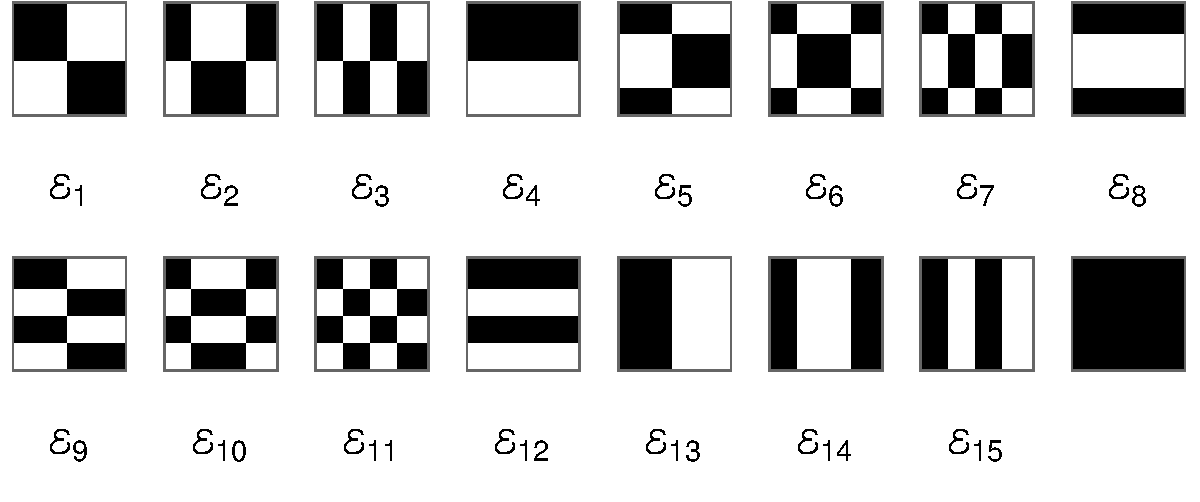
\includegraphics[width=.75\textwidth]{2Q-fundamentals}
  \caption{Generators of 2 qubits.}
  \label{fig:2qubits-generators}
\end{figure}
and concatenation with the patterns is understood as the intersection
of black squares in the patterns of the generators. For example:

\hfill
\begin{tabular}{m{0.8cm} m{.1cm} m{0.8cm} m{.05cm} m{0.8cm}}

\includegraphics[height=1.1cm]{E2}  
& $\bigcirc$ 
& 
\includegraphics[height=1.1cm]{E5} 
& $=$
& 
\includegraphics[height=1.1cm]{E2E5} 
\end{tabular} \hspace{1.3cm}

\hfill
\begin{tabular}{m{0.8cm} m{.1cm} m{0.8cm} m{.1cm} m{0.8cm} m{.1cm} m{0.8cm}}

\includegraphics[height=1.1cm]{E4}
& $\bigcirc$ 
& 
\includegraphics[height=1.1cm]{E2}  
& $\bigcirc$ 
& 
\includegraphics[height=1.1cm]{E5} 
& $=$
& 
\includegraphics[height=1.1cm]{E4E2E5} 
\end{tabular} \hspace{1.3cm}

\hfill
\begin{tabular}{m{0.8cm} m{.1cm} m{0.8cm} m{.1cm} m{0.8cm} m{.1cm} m{0.8cm} m{.1cm} m{0.8cm}}
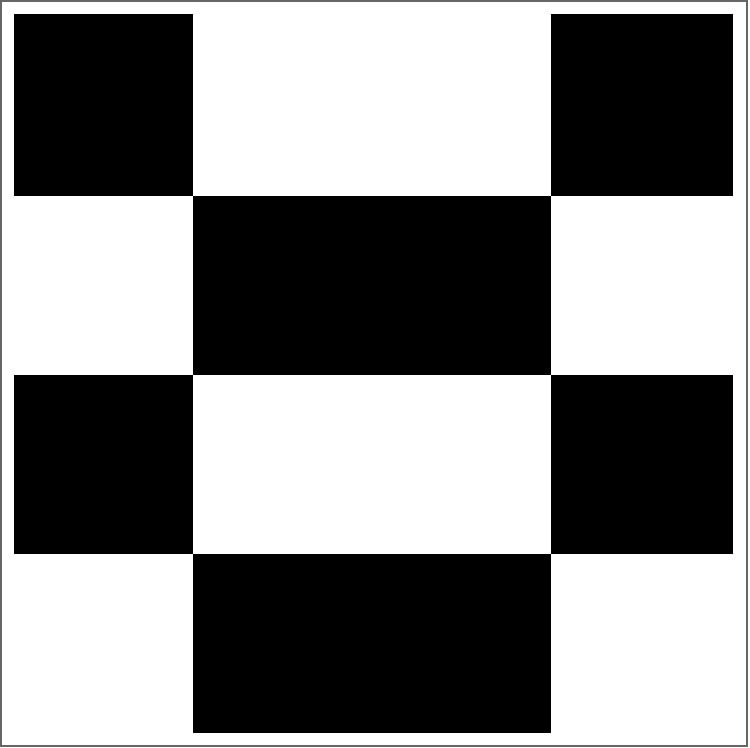
\includegraphics[height=1.1cm]{E12}
& $\bigcirc$ 
& 
\includegraphics[height=1.1cm]{E4}
& $\bigcirc$ 
& 
\includegraphics[height=1.1cm]{E2}  
& $\bigcirc$ 
& 
\includegraphics[height=1.1cm]{E5} 
& $=$
& 
\includegraphics[height=1.1cm]{E12E4E2E5} 
\end{tabular} \hspace{1.3cm}

This shows the idea and that is possible to construct from the generators
in \Fref{fig:2qubits-generators} 
all PCE channels in Figs. from \ref{fig:2q-c1} to \ref{fig:equivalence_class_c44}
\end{itemize}

\section*{Appendix}
\textit{\textbf{Note:}} This section contains
\begin{enumerate}
\item Observations on empirical rules con construct a PCE quantum channel
for 2 and 3 qubits.
\item Comparison with other kind of Pauli operations studied by Ruskai.
\end{enumerate}
The appendix could be skipped without loss of continuity of 
the current observations on our results in the rest of this document.

\begin{itemize}
\item Empirical observations of results for 2 qubits 
led us to some rules that 
patterns showed from \fref{fig:2q-c1} to \fref{fig:2q-c16} obey:
\begin{enumerate}
\item If a component with indices $ij$ is left invariant, then two options are
allowed: \textit{a)} both components with indices $i0$ and $0j$ are left
invariant too, or \textit{b)} both components with indices $i0$ and $0j$ are
erased.
Let us take a look at the next example. 
\begin{center}
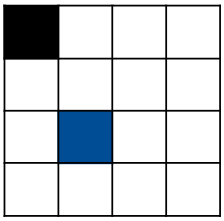
\includegraphics[width=2cm]{ex-2q2c-empiricalRule}
\end{center}
% \hfill \hfill
% \newline
The component with indices 21 in the pattern is left invariant,
then the only options allowed are: \textit{a)} components with indices 01 and
20 are erased, as in this pattern above, or \textit{b)} components 
with indices 01 and 20 are left invariant too, 
as in the following pattern 
\begin{center}
% \newline
% \hfill
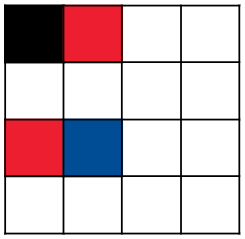
\includegraphics[width=2cm]{ex-2q4c-empiricalRule},
% \hfill \hfill 
% \newline
\end{center}
which is in fact another PCE channel. This rule can be derived using the complete positive condition over the following pattern:
\begin{equation}
\begin{array}{|c|c|c|c|}
\hline
1 & a_1 & 0 & 0 \\ 
\hline
0 & 0 & 0 & 0 \\ 
\hline
a_2 & b & 0 & 0 \\ 
\hline
0 & 0 & 0 & 0\\
\hline
\end{array}
\end{equation}
% \janote{Fin.}

\item Considering only components in the correlation matrix (blue squares): if a component
with indices $ij$ is left invariant and the previous rule is obeyed, then,
in the correlation matrix, remaining components on row $i$ and column $j$ are
erased, and the rest of the components are left invariant by a PCE channel. 
Let's go back to the last pattern in the previous example. This rule 
ensures that components in the correlation matrix outside of row 2 and 
column 1 may be left invariant by a PCE channel, i.e.
\begin{center}
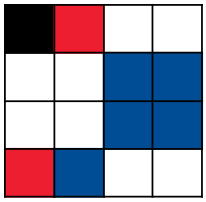
\includegraphics[width=2cm]{ex-2q8c-empiricalRule},
\end{center}
which is another PCE channel.
\end{enumerate}	
Actually, this two simple rules allow us to relate
different equivalence classes. In the previous example we were able to connect 
an element of C${}_2^2$ to one of C${}_3^4$, to another one of
C${}_2^8$.

\item The action of a PCE channel on every subsystem must be another
PCE channel. 
This can be seen from the patterns in \fref{fig:2q-c1} to \fref{fig:2q-c16}.
Recall that red squares represent components of local Bloch vectors 
and blue squares represent correlations shared between qubits. 
Then, it may be noted in the first column and first row of every
pattern there is a 1-qubit PCE quantum channel of the form of \fref{fig:1q-ccs}.
% \janote{\h{Fin}}
\end{itemize}
% }}}
\subsection*{3 qubits} % {{{

Recall that for 3 qubits system we have numerically analyzed only maps that
leave invariant 1, 2, 3, 4, and 64 components in $\rho$. Therefore, results
presented in this section are preliminary. Maps that are PCE channels follow the same
features of 2-qubits system. Not all 3-qubits PCE channels 
will be shown as in
the previous section, but only one element of every equivalence class found.
Elements in equivalence classes are connected via particle swaps and
permutation of individual components.

\subsubsection*{1-invariant-component maps} % {{{
The only map that leaves invariant 1 component in $\rho$ is the completely
depolarizing channel, and it is trivially a PCE channel.
\begin{figure}[H]
	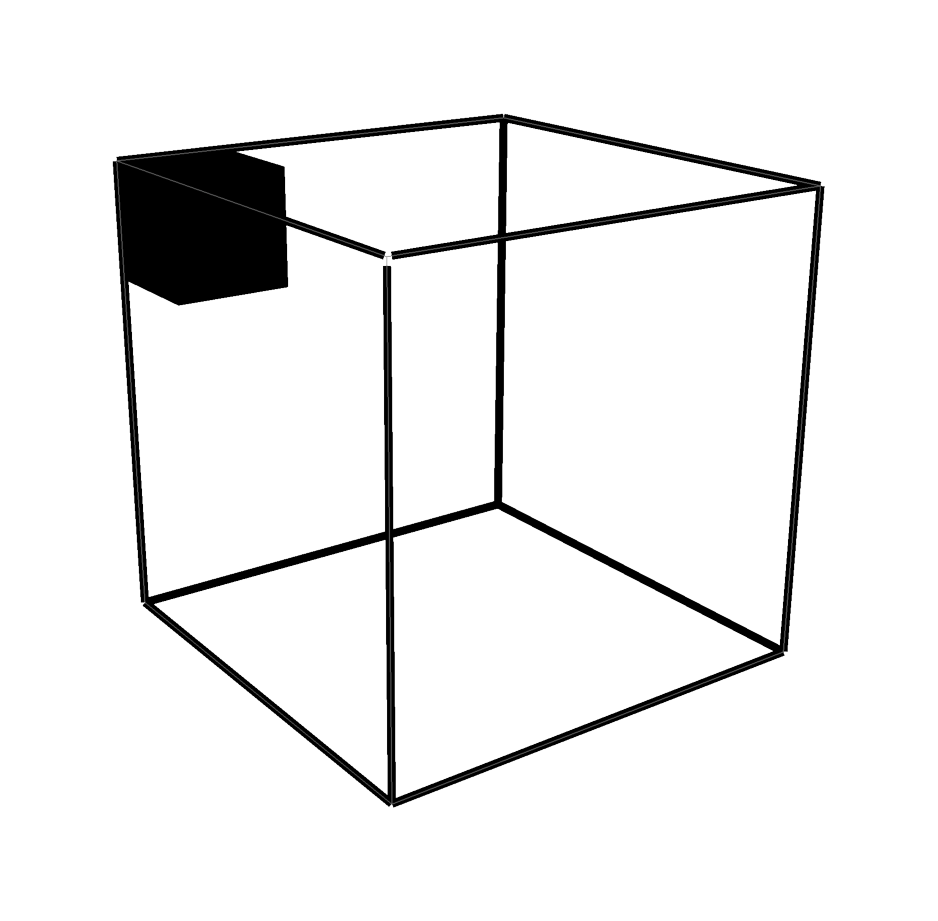
\includegraphics[height=4cm]{3q-1c}
	\caption{Completely depolarizing channel for 3 qubits.}
	\label{fig:QC-3q-1c}
\end{figure}
% }}}
\subsubsection*{2-invariant-components maps}% {{{
All 63 maps that leave invariant 2 components in $\rho$ are 
PCE channels. It's important to mention that in the 2-qubits case all 
2-invariant-components maps are PCE channels, too. We can distinguish
3 equivalence classes: quantum channels that leave invariant
\begin{enumerate}
	\item any component of a local Bloch vector,
	\item any correlation between any pair of qubits,
	\item any correlation between all qubits in the system.
\end{enumerate}
\begin{figure}[H]
	\centering
	\hfill \hfill
	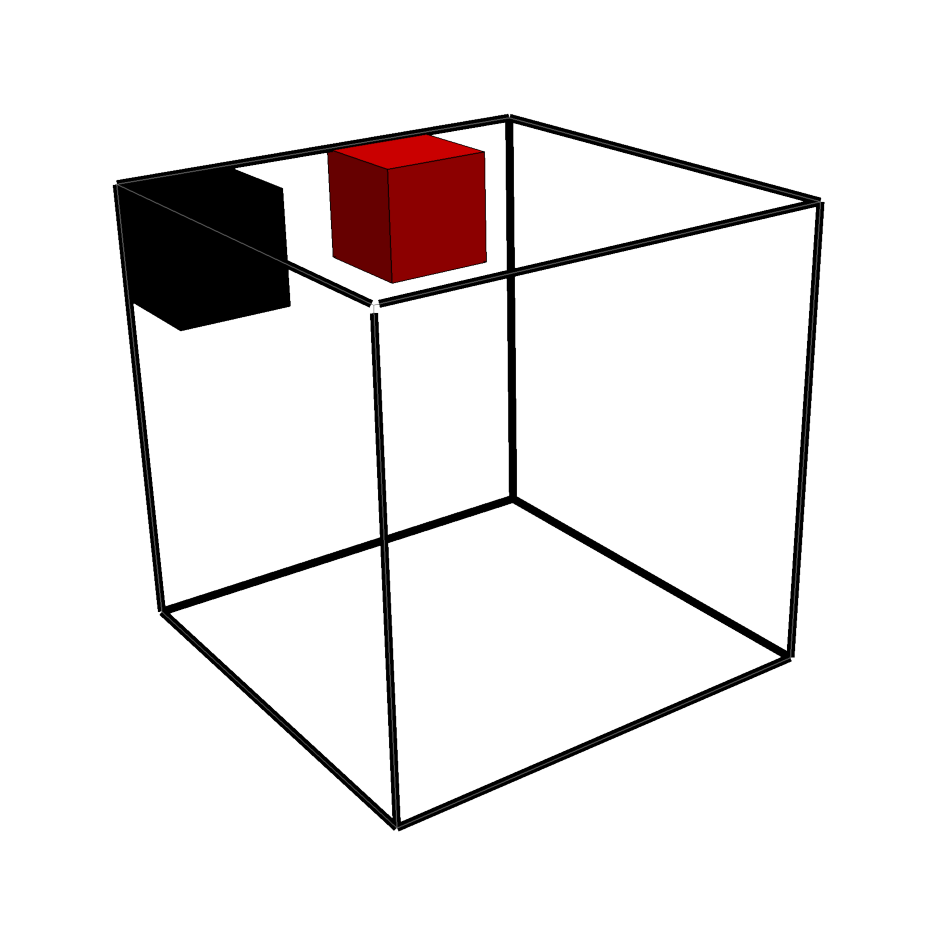
\includegraphics[height=4cm]{3q-2c-1}
	\hfill
	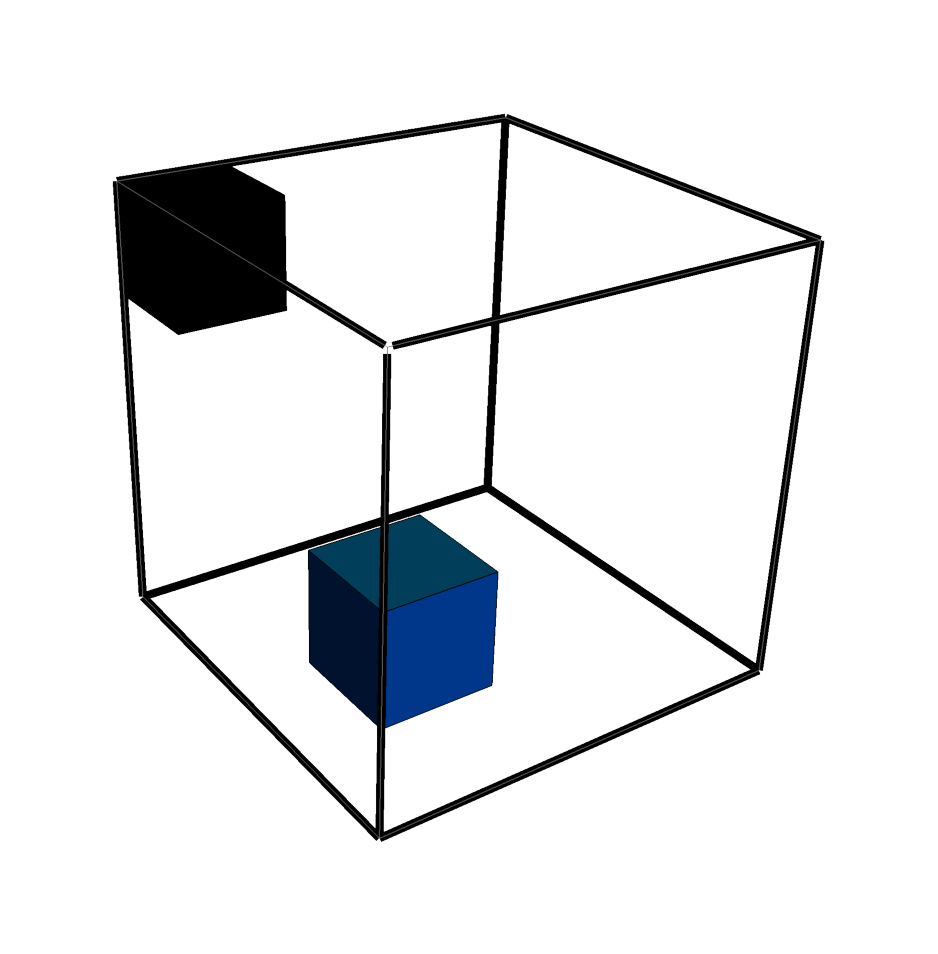
\includegraphics[height=4cm]{3q-2c-2}
	\hfill
	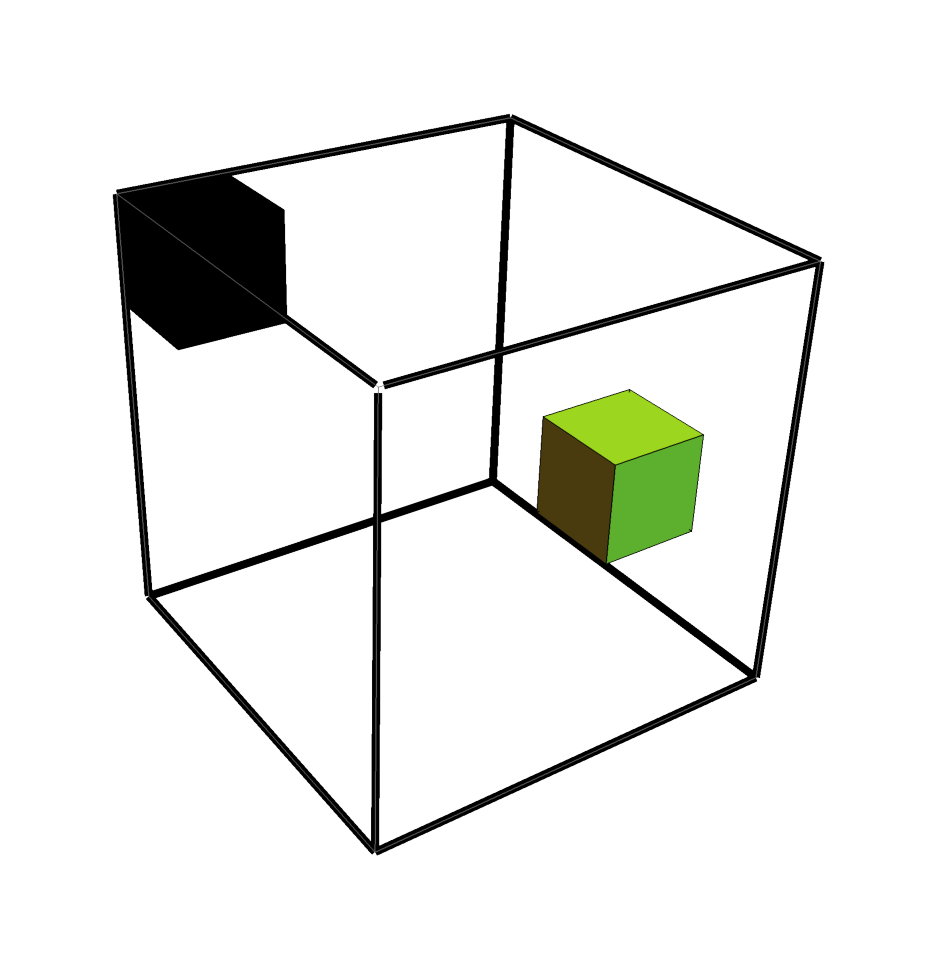
\includegraphics[height=4cm]{3q-2c-3}
	\hfill \hfill
	\caption{3-qubits 2-components-invariant PCE channels. 
	One element of each of the 3 equivalence classes 
	(from left to right): leaves invariant one component of any local
	Bloch vector, one correlation between any pair or qubits, and 
	one correlation between all qubits in the system.}
	\label{fig:QC-3q-2c}
\end{figure}

% }}}
\subsubsection*{3-invariants-component maps} % {{{
No PCE channels were found in the set of all maps that leave
3 components invariant in $\rho$.
% }}}
\subsubsection*{4-invariant-components maps} % {{{
There are 39,711 maps that leave invariant 4 components in $\rho$, 651
are PCE channels and may be classified in 10 equivalence classes.
One arbitrary element in each class is shown in \fref{fig:QC-3q-4c}. 
We understand how to infer 5 out of the 10 equivalence classes 
from 1 and 2-qubits PCE channels, as it will be discussed.

On top of \fref{fig:QC-3q-4c} the first 4 elements
(from left to right) correspond to PCE channels that are separable
in a 1 or 2 qutbis PCE channel acting on any subsystem 
and a completely depolarzing channel acting on the rest of the system.
The fifth and last element on top of the figure may be understood invoking    
an extension for 3 qubits of one of the empirical rules presented 
for 2 qubits. The extensions of those rules will be discussed at
the end of this section. 
PCE channels belonging to equivalence classes of bottom elements in 
the figure are such that we still cannot infer them with our 
previous results.

\begin{figure}[H]
	\centering
	\hfill \hfill
	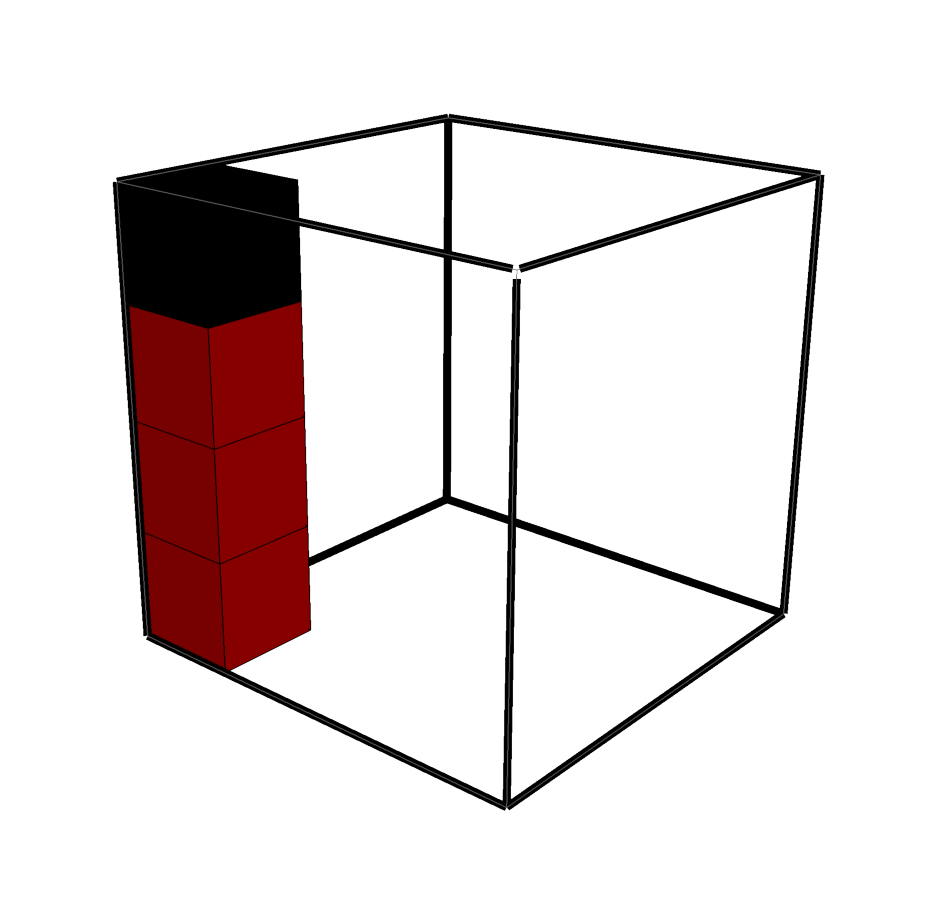
\includegraphics[height=3cm]{3q-4c-si-1}
	\hfill
	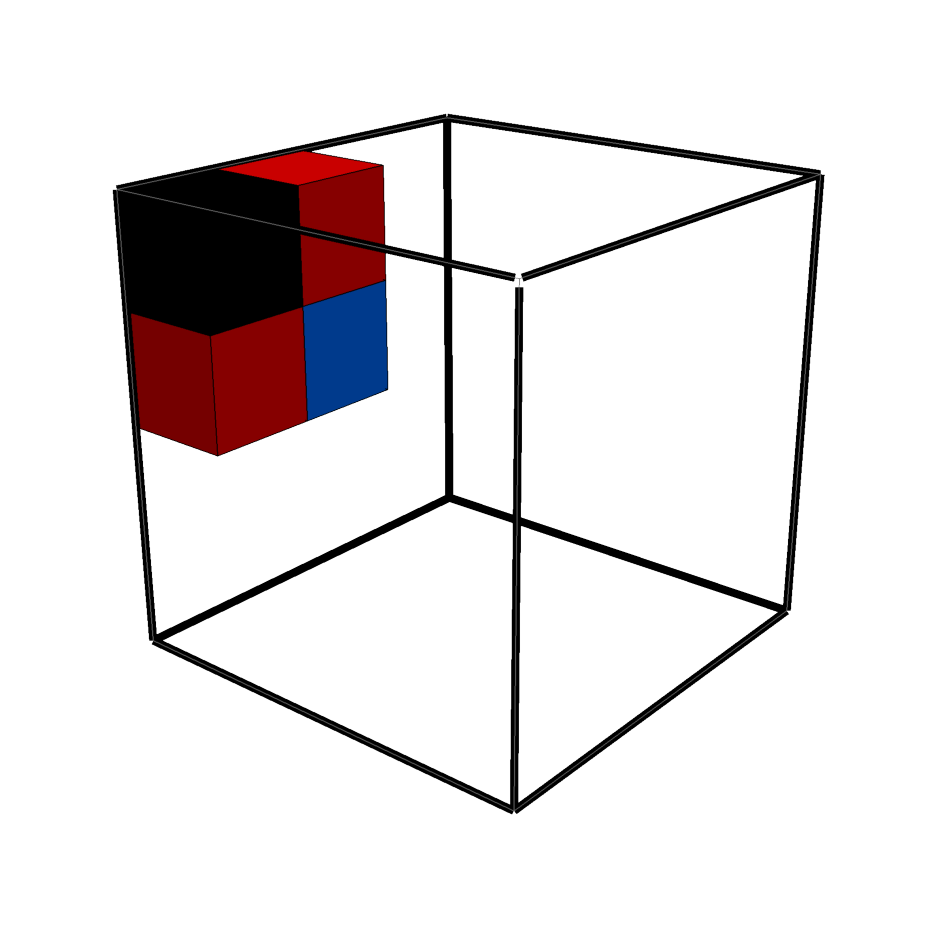
\includegraphics[height=3cm]{3q-4c-si-2}
	\hfill
	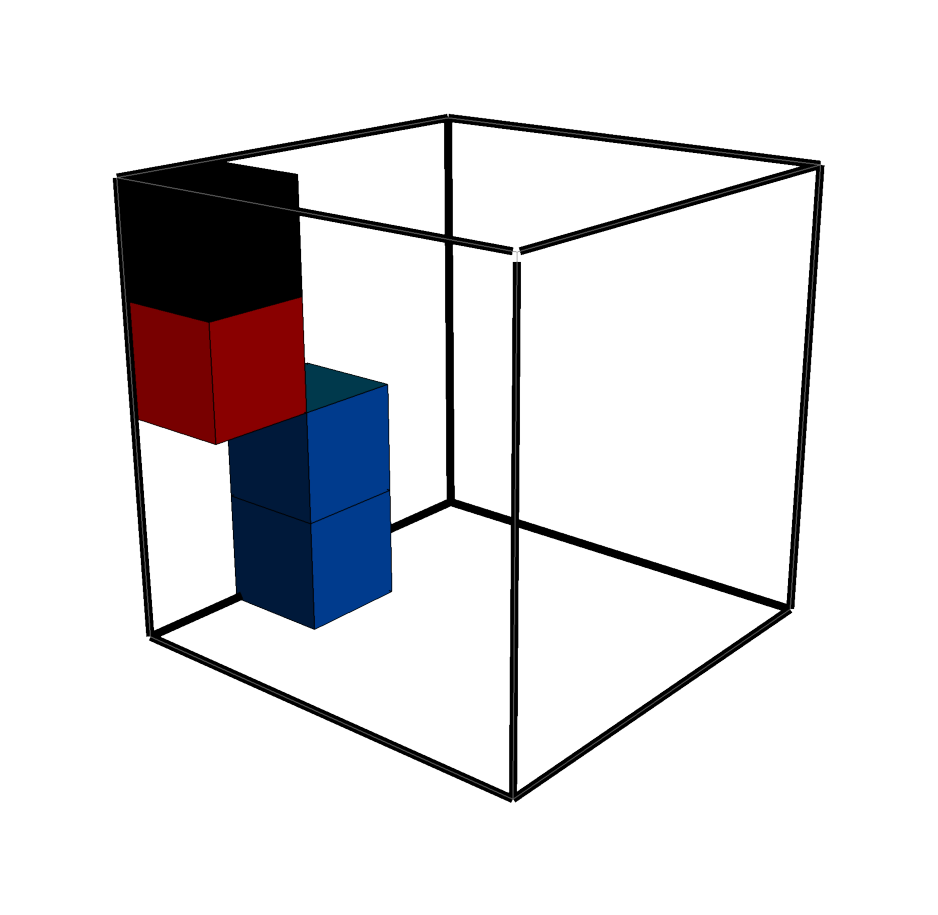
\includegraphics[height=3cm]{3q-4c-si-3}
	\hfill
	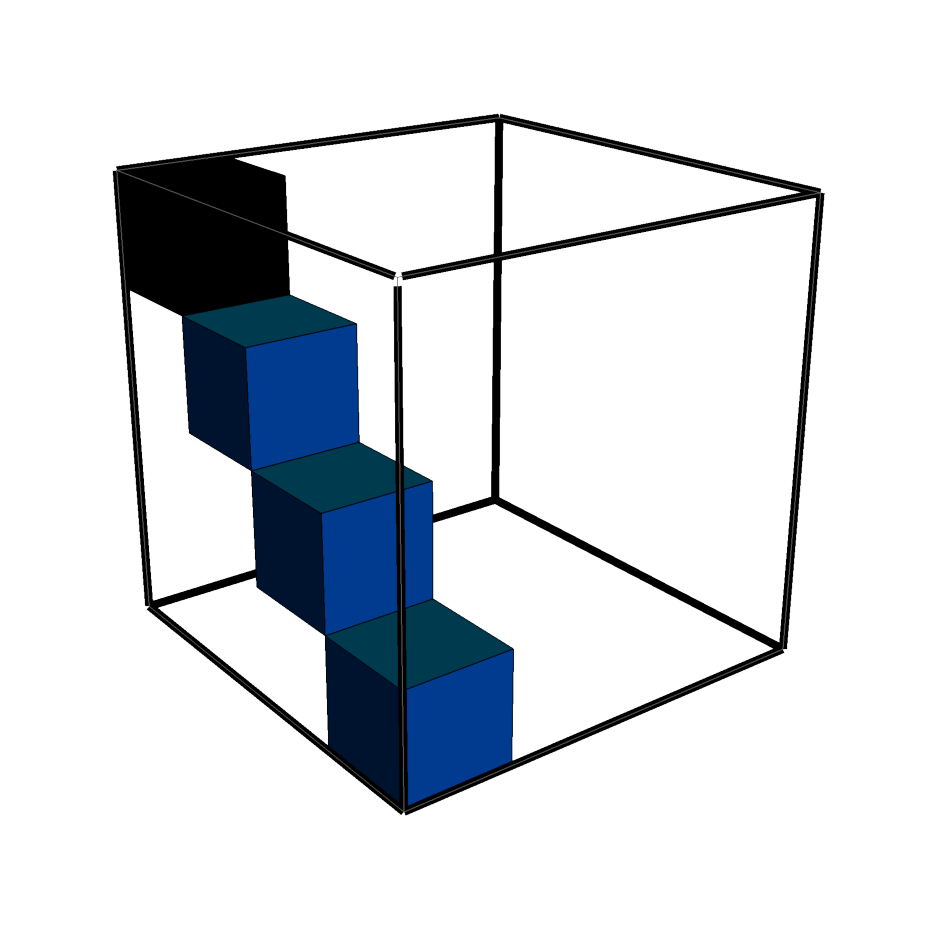
\includegraphics[height=3cm]{3q-4c-si-4}
	\hfill
	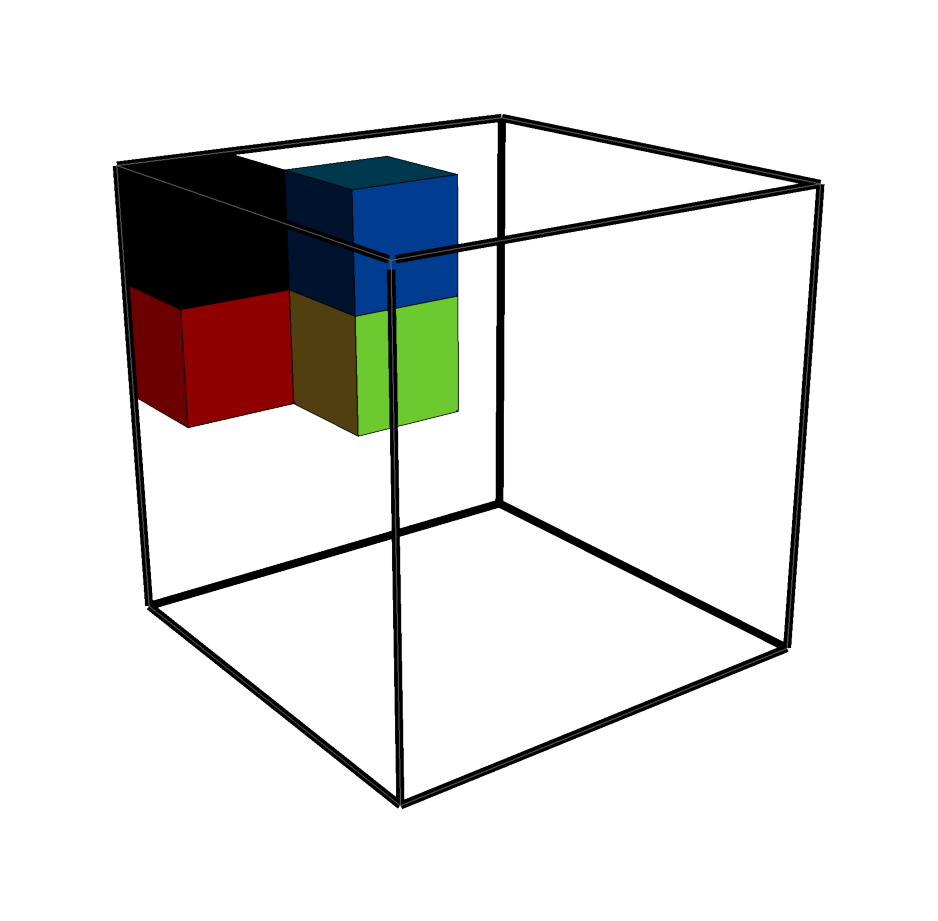
\includegraphics[height=3cm]{3q-4c-si-5}
	\hfill
	\vfill
	\hfill
	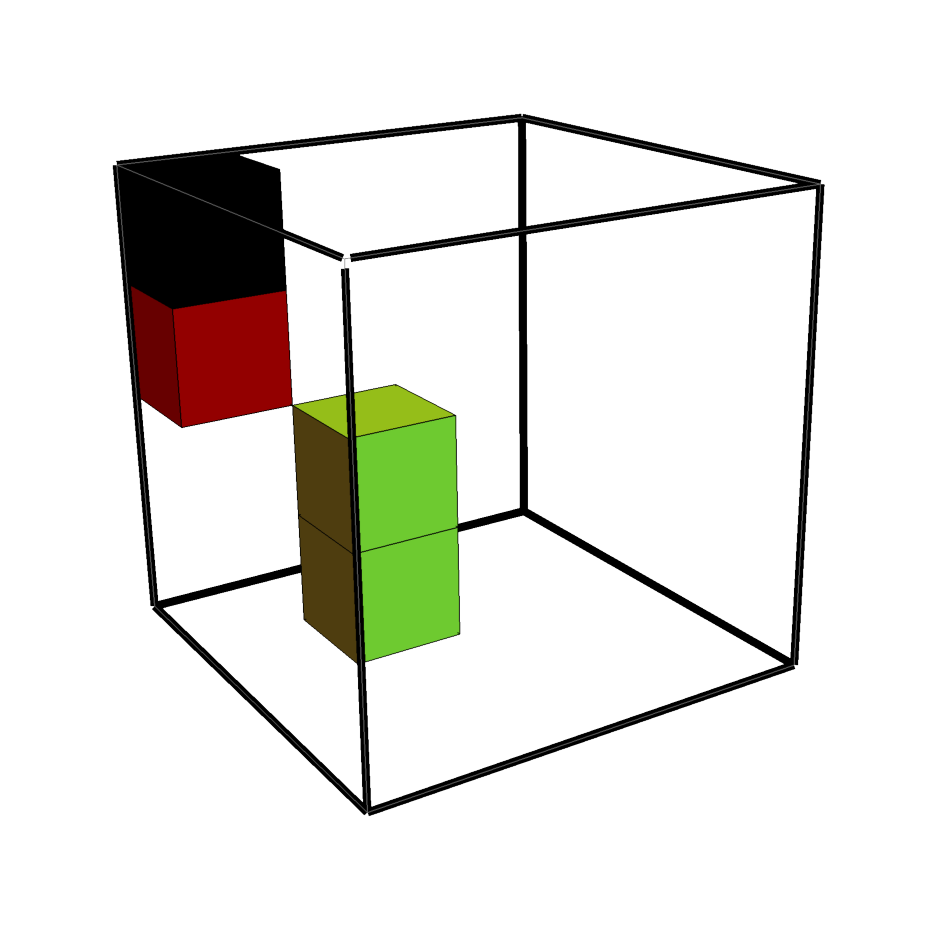
\includegraphics[height=3cm]{3q-4c-no-1}
	\hfill
	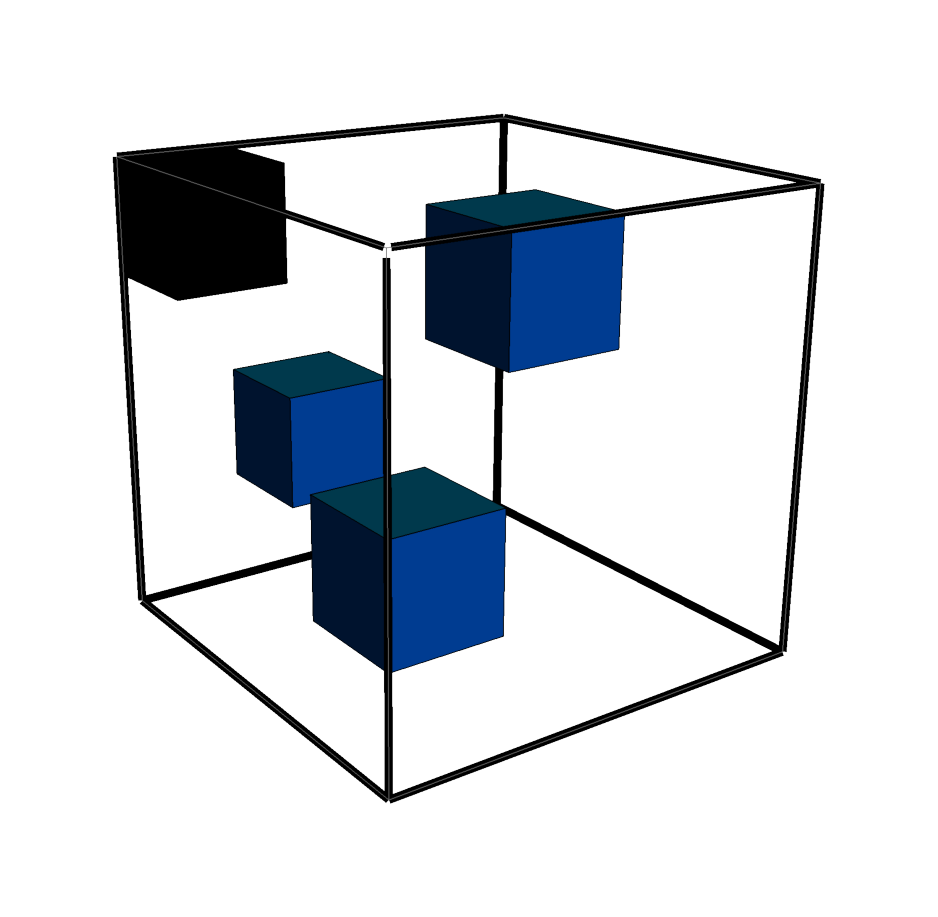
\includegraphics[height=3cm]{3q-4c-no-2}
	\hfill
	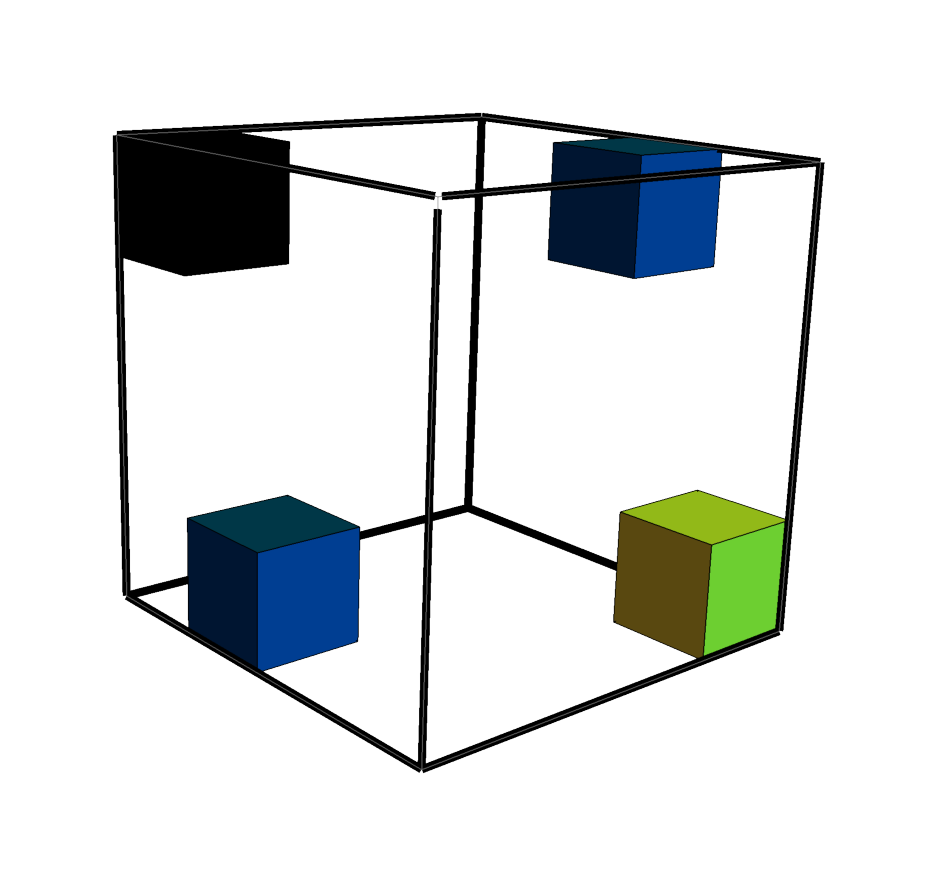
\includegraphics[height=3cm]{3q-4c-no-3}
	\hfill
	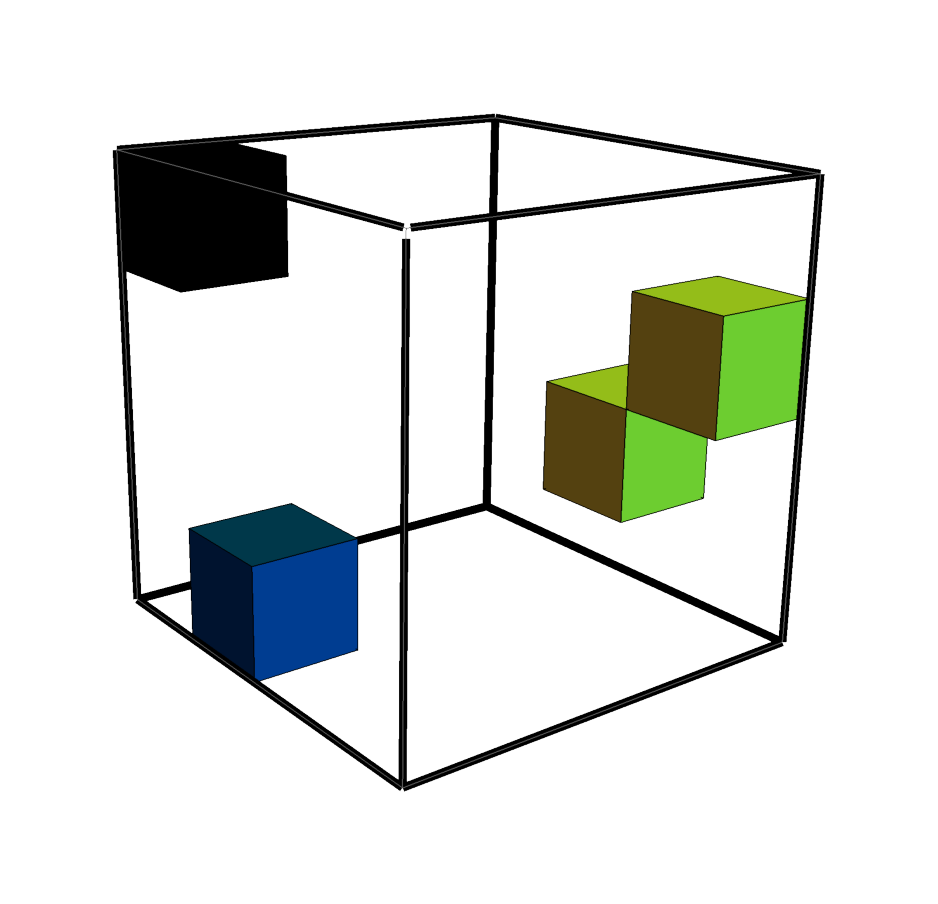
\includegraphics[height=3cm]{3q-4c-no-4}
	\hfill
	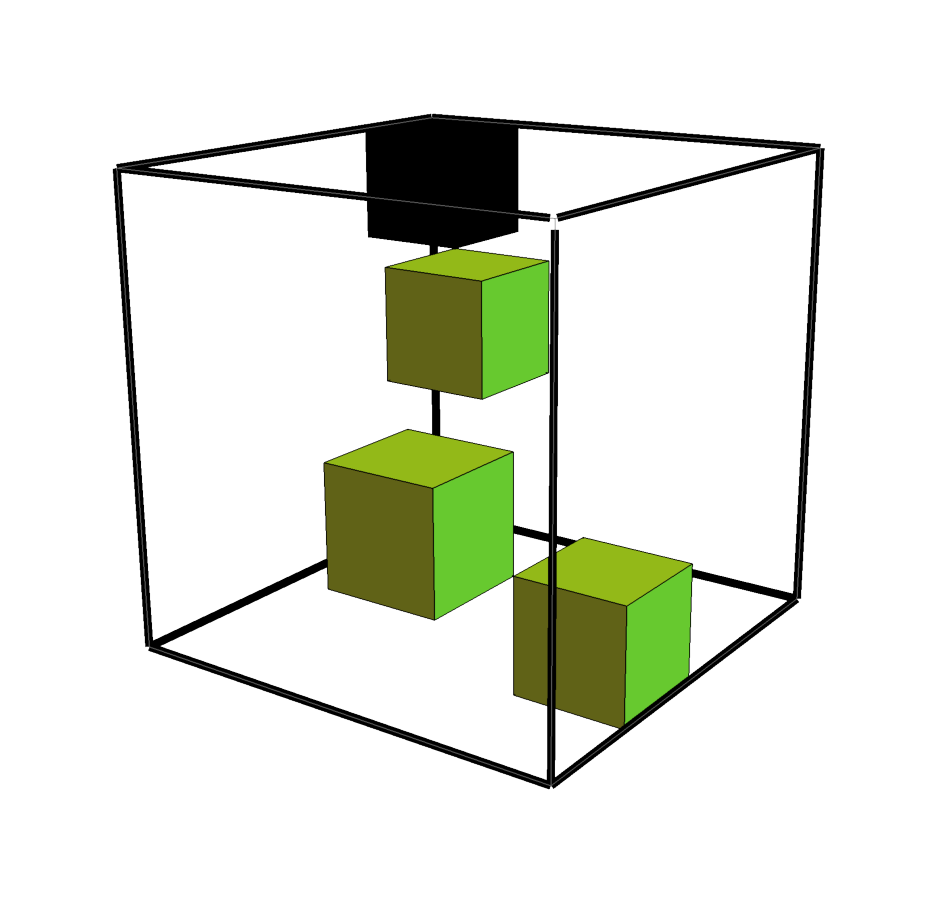
\includegraphics[height=3cm]{3q-4c-no-5}
	\hfill \hfill
	\caption{3-qubits 4-components-invariant PCE channels. 
	One element of every of the 10 equivalence classes.}
	\label{fig:QC-3q-4c}
\end{figure}
% }}}
% Rules for 3 qubits {{{
The empirical rules already presented for 2 qubits can be 
formulated for 3 qubits as follows:
\begin{itemize}
	\item A component with indices $ijk$ (all different from zero) is
	left invariant by a PCE channel if and only if 
	one of the cases is followed:
	\begin{enumerate}
		\item Components $ij0$, $0jk$, $i0k$, $i00$, $0j0$, and
		$00k$ are erased.
		\item Components $i00$ and $0jk$ are also left invariant.
		\item Components $0j0$ and $i0k$ are also left invariant.
		\item Components $00k$ and $ij0$ are also left invariant.
		\item Components $ij0$, $0jk$, $i0k$, $i00$, $0j0$, and
		$00k$ are also left invariant.
	\end{enumerate}
	It can be noted that the element in the right upper corner of 
	\fref{fig:QC-3q-4c} is understood as one of the cases 2-4 of this item.
	\item Considering only components that correspond to correlations between
	3 qubits in the system (green cubes): if a little cube 
	with indices $ijk$ (all different from zero) is left invariant 
	and any of the cases of the previous rule is obeyed, 
	then the remaining components on columns $i$, $j$, and $k$ are
	erased and the rest of components in the correlation tensor 
	are left invariant by a PCE channel. 
\end{itemize}
Let us consider an example to make use of both empirical rules. If we 
begin with an element of the same equivalence class as the second
element on top of \fref{fig:QC-3q-4c}, then we make use of one of 
the cases 2-4 of the first empirical rule for 3 qubits and get the PCE channel below.
\begin{center}
	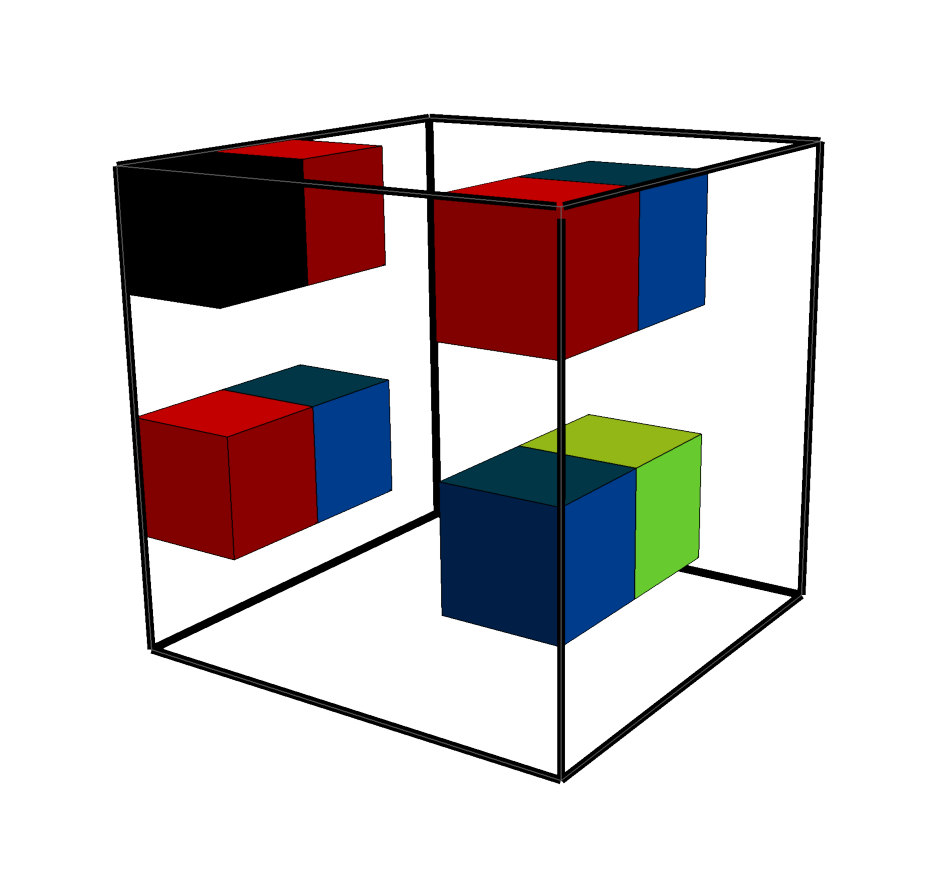
\includegraphics[width=4cm]{3q-8c-je}.
\end{center}
Finally, we make use of the second rule to left invariant only components
corresponding to correlations between all qubits in the system (green cubes)
and get another PCE channel (pattern below).
\begin{center}
	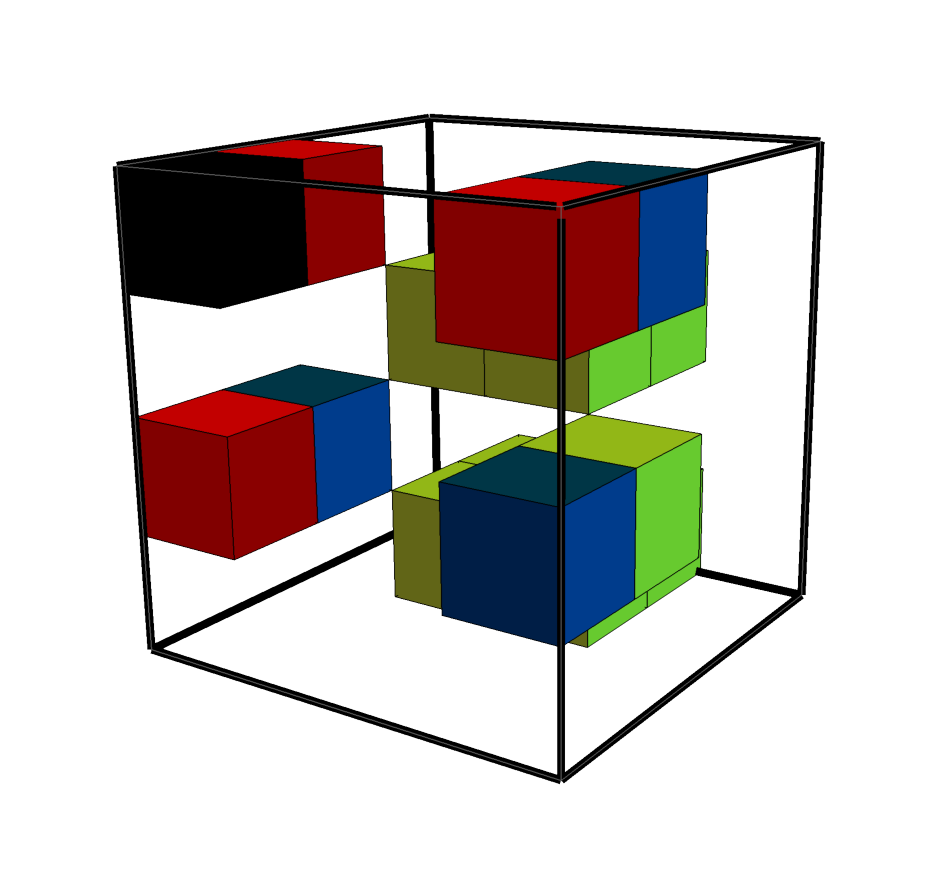
\includegraphics[width=4cm]{3q-8c}
\end{center}
What we have done is start with a PCE channel that leaves 4 invariant
components, make our way trough a 8-invariant-components PCE channel and 
finally arrive at a 16-invariant-components PCE channel.

In principle, the rainbow hypothesis ensures the correspondence between  
the channels we have found and channels that leave invariant 16, 32 and 64
components. The empirical rules for 3 qubits provide one way to \textit{travel}
from a $k$-components-invariant quantum channel to a
$(2n-k)$-components-invariant channel.
It is sufficient to found one element in an 
equivalence class because the rest of the elements are found 
by particle swaps and permutation of individual components.
% }}}
% }}}
% }}}
\section*{Are this channels a subset of Pauli diagonal channels constant on axes?} % {{{
We explored if PCE channels are contained within the set of Pauli diagonal
channels constant on axes \cite{nathanson2007pauli}. Let us call them
$\mathcal{R}$. For 2 qubits, we concluded that Kraus rank $4$ 
PCE channels are the only candidates to
be in $\mathcal{R}$, in fact we are convinced that all of them are in, but are
still working in the proof. 
To see this let us analyze the action of maps in $\R$ 
on arbitrary density matrices
\begin{align}
	\rho \longmapsto \frac{1}{d}\qty[\1 + \sum _{J=1}^{d+1} \lambda_J
	\sum _{j=1}^{d-1}	v_{Jj}W_J^j],
	\label{eq:ruskai-action}
\end{align}
where $\lambda_J$ are the eigenvalues of a given map, and operators $W_J$ are unitaries defined as
\begin{equation}
	W_J = \sum _{k=1}^{d}\omega^k \dyad{\psi_k^J}{\psi_k^J}, 
\end{equation}
where sets of vectors $\qty{\ket{\psi_k^J}}_k$ with $J=1,\dots, 1+d$ are mutually unbiased basis (MUB) over $\mathbb{C}^d$, and $\omega = e^{2\pi i/d}$. There are $d^2-1$ unitaries generated with the powers of the $W_J$s, i.e.
$\qty{W_J^m}_{m=1,\ldots,d,J=1,\ldots,d+1}$. They, together the identity matrix, form a basis in the space of $d\times d$ matrices.
%\fxnote{Por fas
%corrige la argumentacion a partir de la modificacion a la ecuacion} 

%\fxnote{JA, ojo
%que los $W_J$ generan un grupo ciclico, mas no generadores de MUBs, uno
%construye los $W_J$ usando MUBs!. Por fas mejor mete la definicion de $W_J$.}
 

To examine if PCE channels are contained in $\R$ let us consider
the rank of both maps and discuss how only a subset of PCE channels
could be in $\R$. Our results show that PCE channels have 
a power-of-2 rank. On the other hand, from \eqref{eq:ruskai-action} it
can be seen that the rank of a map in $\R$ is 1 plus 
the number of all $\lambda_J$ different from zero. Notice that eigenvalues $\lambda_J$ have multiplicity $d-1$, for each $J$. Consequently, the allowed matrix ranks 
of maps in $\R$ are $1 + k(d-1)$, where $k = 1,2,\ldots,d+1$. It follows
that a \textit{necessary} condition for maps in $\R$ and PCE channels to have the 
same rank is that
\begin{align}
	\hspace{2cm}2^j&=1 + k(2^{2n}-1),	\hspace{1.5cm} j=0,1,\ldots,2n
\end{align}
is always true for some $k\in \mathbb{Z^+}$, and $n$ the number 
of qubits. If we take $n=2$ and $j=3$ 
(2 qubits, $2^3$ components invariant)
\begin{align}
	k&= \frac{2^3-1}{2^{2\qty(2)}-1}=\frac{7}{15}.
\end{align}
Therefore the rank of a PCE channel may not be the same of any map in $\R$.
Then, there are PCE channels that cannot be in $\R$, like
all 8-components-invariant PCE channels, as shown in the previous example. 


%% }}}
%\section*{To-do} % {{{
%In order to fully understand our results and generalize this kind of maps 
%for $n$ qubits we propose the following:
%\begin{enumerate}
%\item Investigate the Kraus operator representation of this quantum channels.
%\item Investigate the Schmidt spectrum of the Choi matrix.
%\item Investigate the Jamiolkowski isomorphism to find an equivalence between
%CP and the empirical rules listed previously.
%\item Use our current results to propose an efficient way to do numerical
%analysis to find 3-qubit quantum channels that leave 8 components invariant.
%\end{enumerate}
%% }}}
\bibliographystyle{unsrt}
\bibliography{references}
\vfill

\end{document}
